%
% Dokumentation
%

% Allgemeine Dokumenteigenschaften
\documentclass[a4paper,			% Druck auf DIN A4-Papier.
numbers=enddot,					% Die Kapitel bekommen einen Punkt.
chapterprefix=false,			% Das Wort "Kapitel:" wird gelöscht.
12pt,							% 12pt ist die Normalschriftgröße, weitere Möglichkeitenn sind 10pt oder 11pt.
pointlessnumbers				% Nummerierungen in den Kapiteln haben keinen finalen Punkt zb 1.1 statt 1.1.
]							
{scrreprt}  					% Dokumentart.

\setkomafont{chapter}{\Large}
\setkomafont{section}{\large}

% Präambel: Parameter die sich auf das Gesamte Dokument auswirken.
\usepackage{geometry}
\usepackage{float}
\usepackage[ngerman]{babel}				% "Neue" Deutsche Rechtschreibung
\usepackage{textcomp}					% Aktiviert das Eurosymbol. (Im Text schreiben mit \texteuro)
\usepackage[utf8]{inputenc}				% Direkte Eingabe von Umlauten im Text. (Dieser Code läuft nicht überall)
\usepackage{graphicx}					% Ermöglicht das anzeigen von Bildern
%\usepackage{babelbib}					% Für verschiedene Deutsche Stile des Literaturverzeichnis
\usepackage{apacite}
%\usepackage[babel, german=guillemets]{csquotes}
\usepackage[babel,german=quotes]{csquotes}
\usepackage{amsmath,amssymb}			% Das Mathe Paket "American Mathematic Society" laden
\usepackage[printonlyused]{acronym}		% Paket für das Abkürzungsverzeichnis
\usepackage{fancyhdr}					% Fancyhdr zum Nutzen von Kopf und Fußzeilen mit voreingestellten Formatierungen
\usepackage{xcolor}						% Verschiedene Farben sind direkt als white usw nutzbar
\usepackage{epstopdf}					% eps Postscript Dateien können direkt eingefügt werden
\usepackage{tocstyle}					% Das Inhaltsverzeichnis lässt sich konfigurieren
\usepackage{listings}					% Ermöglicht das Einfügen von Quellcode mit Kommentarhighlighting und Nummerierung aussen
\usepackage{subfig}						% 2 Bilder nebeneinander
\usepackage{chngcntr}
\usepackage{tabularx}
\counterwithout{figure}{chapter} 




% Kapitel, Bilder, Abkürzungen usw werden zu Links, ohne roten Rahmen. DAS FUNKTIONIERT NICHT MIT APACITE!!!!
%\usepackage[plainpages=false,
%pageanchor=false,
%linkbordercolor=white,					% Die Rahmen werden weiß und sind somit nicht mehr im PDF sichtbar
%pdfpagelabels]
%{hyperref}								% Inhaltsverzeichnis wird als Lesezeichen im Adobe Reader angezeigt	

% Absatz-Einstellungen
\geometry{a4paper,
left=20mm,
right=20mm,
top=2.5cm,
bottom=2.5cm}
\parindent0ex							% Oberster Satz eines Absatzes wird NICHT eingerückt!
\parskip1.4ex plus0.2ex minus0.2ex


% Kopf und Fußzeile einbinden und festlegen.
\pagestyle{fancy}									% Eigenen Seitenstil verwenden
\fancyhf{} 											% clear all header and footer fields
\renewcommand{\headrulewidth}{1pt}					% Die Dicke der Kopfzeilen-Trennline wird auf 1pt festgelegt
\renewcommand{\footrulewidth}{1pt}					% Die Dicke der Fusszeilen-Trennline wird auf 1pt festgelegt
\fancypagestyle{plain}{}
\fancyhead[R]{}										% Kopfzeile Rechts
\fancyfoot[R]{\thepage}								% Fusszeile Rechts

% Inhaltsverzeichnis anpassen.
\usetocstyle{allwithdot}				% Fällt den Leerraum mit Punkten auf
\setcounter{tocdepth}{1}

% Das eigentliche Dokument.
\begin{document}

% Dokumentenweite Einstellungen und Kommandos
\nonfrenchspacing
\newcommand{\FigRef}[1]{Abbildung \ref{#1} auf Seite \pageref{#1}}
\newcommand{\TabRef}[1]{Tabelle \ref{#1} auf Seite \pageref{#1}}
\renewcommand*{\chapterheadstartvskip}{\vspace*{0pt}}					% Abstand vor Kapitelnamen
\renewcommand*{\chapterheadendvskip}{\vspace{1cm}}						% Abstand nach Kapitelnamen
\setlength{\headheight}{30pt}											% Höhe der Kopfzeile festlegen
\setlength{\footskip}{30pt}												% Abstand von Text zu Fusszeile festlegen

% Titelseite
%
% Dokumentation
%

% 1. Seite
\thispagestyle{empty}

\begin{figure}
\flushright						% rechtsbündig

\includegraphics[width=5cm,clip=]{Bilder/HHN_ab_40_mm_4c_pos4}\\
\end{figure}

\vspace*{1.0cm}

\begin{center}
{\Huge Benutzerdokumentation\\
\vspace{0.1cm} 
für die Software\\
\vspace{0.1cm} 
\textbf{we}Factor}

\vspace{3.0cm}

	{\Large Als Projektarbeit für die Vorlesung\\
\vspace{0.1cm}
	Labor für Softwareentwicklung und Project Skills\\
\vspace{0.1cm}
	im Studiengang Software Engineering\\
\vspace{0.1cm}
	der Hochschule Heilbronn\\

}
\end{center}

\vspace*{4.5cm}





Autor:\\
{\Large
Florian Wohlgemuth\\

 }
\vspace{1,5cm}
Heilbronn, \today
%\textbf{FIRMA}, Str. 1, 12345 Ort\\
%Betreuer: Dr. Jemand\\

\fancyhf{} 											% clear all header and footer fields
\renewcommand{\headrulewidth}{1pt}					% Die Dicke der Kopfzeilen-Trennline wird auf 1pt festgelegt
\renewcommand{\footrulewidth}{1pt}					% Die Dicke der Fusszeilen-Trennline wird auf 1pt festgelegt
\fancypagestyle{plain}{}
\fancyhead[R]{}										% Kopfzeile Rechts
\fancyfoot[R]{\thepage}								% Fusszeile Rechts

\pagenumbering{Roman}  								% Die Verzeichnisse werden entsprechend mit römischen Seitenzahlen beschriftet

% +++++++++++++++++++++++++++++++++++++ab hier beginnen (vor dem inhaltsverzeichnis)

% Aenderungshistorie
\begin{tabularx}{\textwidth}{|l|X|l|l|} \hline
       \textbf{Version}  	& \textbf{Name}   	& \textbf{Kapitel}  & \textbf{Datum}\\ \hline
       0.1           		& Florens Hückstädt & Kapitel 1 		& 31.12.20014\\
        \hline
\end{tabularx}

% Inhaltsverzeichnis
%
% Dokumentation
%

% Kapitel dem Inhaltsverzeichnis hinzufügen
\addcontentsline{toc}{chapter}{Inhaltsverzeichnis}			% 1. Argument {toc} = Table Of Contents
															% 2. Argument {chapter} = Ebene bestimmen!
															% 3. Argument {Name} = Name des Eintrags
\noindent

\tableofcontents
	\thispagestyle{plain}
	\newpage				% Neue Seite erzwingen

% Abkürzungsverzeichnis
%
% Dokumentation
%

% Kapitel dem Inhaltsverzeichnis hinzufügen
\addcontentsline{toc}{chapter}{Abkürzungsverzeichnis}			% 1. Argument {toc} = Table Of Contents
																% 2. Argument {chapter} = Ebene bestimmen!
																% 3. Argument {Name} = Name des Eintrags
\noindent

\thispagestyle{plain}

\chapter*{Abkürzungsverzeichnis}
\begin{acronym}[PP]
\acro{JRE}{Java Runtime Environment}



\end{acronym}


% Abbildungsverzeichnis
%
% Dokumentation
%

% Kapitel dem Inhaltsverzeichnis hinzufügen
\addcontentsline{toc}{chapter}{Abbildungsverzeichnis}			% 1. Argument {toc} = Table Of Contents
																% 2. Argument {chapter} = Ebene bestimmen!
																% 3. Argument {Name} = Name des Eintrags
\noindent

\thispagestyle{plain}


\listoffigures



\pagenumbering{arabic}  							% Der folgende Text wird mit arabischen Zahlen beschriftet



% Kapitl Überblick

\thispagestyle{plain}

\chapter{Einführung}
WeFactor ist eine Anwendung, die zur Refaktorisierung von Code-Stücken vieler verschiedener Programmiersprachen dient. Es ist gewährleistet, dass Code immer weiter optimiert werden kann und dieser leicht und schnell auffindbar ist. 

Im Folgenden werden alle Funktionen der Anwendung schrittweise beschrieben. Alle Schritte werden mit Screenshots bildlich dargestellt. Auf diesen Screenshots weisen große grüne Pfeile darauf hin, welche Buttons gedrückt werden müssen um in der Anwendung zum nächsten Schritt zu kommen, welcher weiter im Dokument wieder als Screenshot dargestellt wird. Elemente die mit Nummerierungen versehen sind, werden weiter im Text genauer beschrieben.

Es ist möglich die Benutzerdokumentation von Anfang bis Ende durchzulesen und hat somit alle Funktionen kennengelernt, ebenso ist es auch möglich direkt zu einzelnen Funktionen zu springen die man gerade braucht, da es für jede Funktion ein eigenes Kapitel gibt.
Die Hilfefunktion ist auch jeder Zeit in der Anwendung aufrufbar. Um diese aufrufen zu können, muss man lediglich rechts oben auf seinen Benutzername klicken und den \glqq Help\grqq -Button betätigen. 



\chapter{Die Erstellung eines Accounts}
Wenn sie die Anwendung installiert und gestartet haben, wie in der Installationsdokumentation beschrieben, haben Sie nun die Möglichkeit einen neuen Account zu erstellen oder mit einem bereits bestehenden, auf der Anwendung erstellten Account, anzumelden. Ebenso ist es möglich sich mit seinem Google+ Account anzumelden.

\begin{figure}[H]
    \centering
    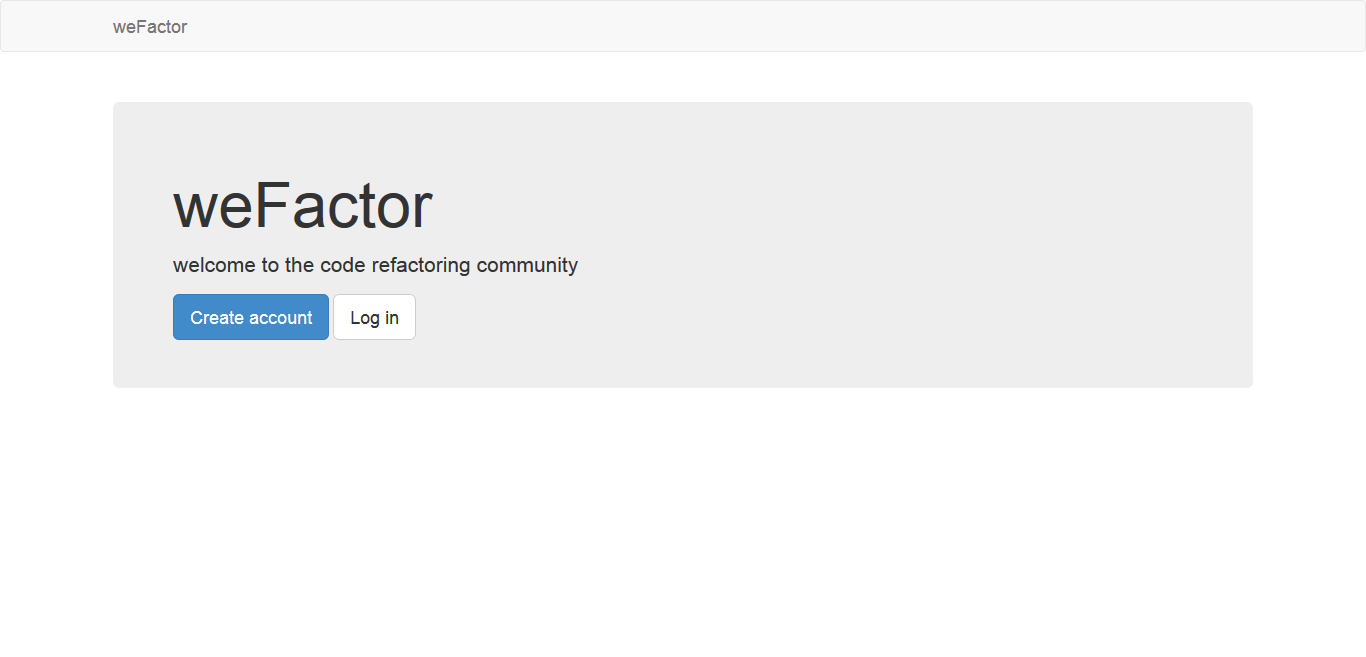
\includegraphics[width=0.8\textwidth]{Bilder/1.png}
    \caption{Startseite}
    \label{fig:startseite}
\end{figure}


Um auf die Seite der Accounterstellung zu gelangen, wird auf den Button „Create Account“ geklickt.

\begin{figure}[H]
    \centering
    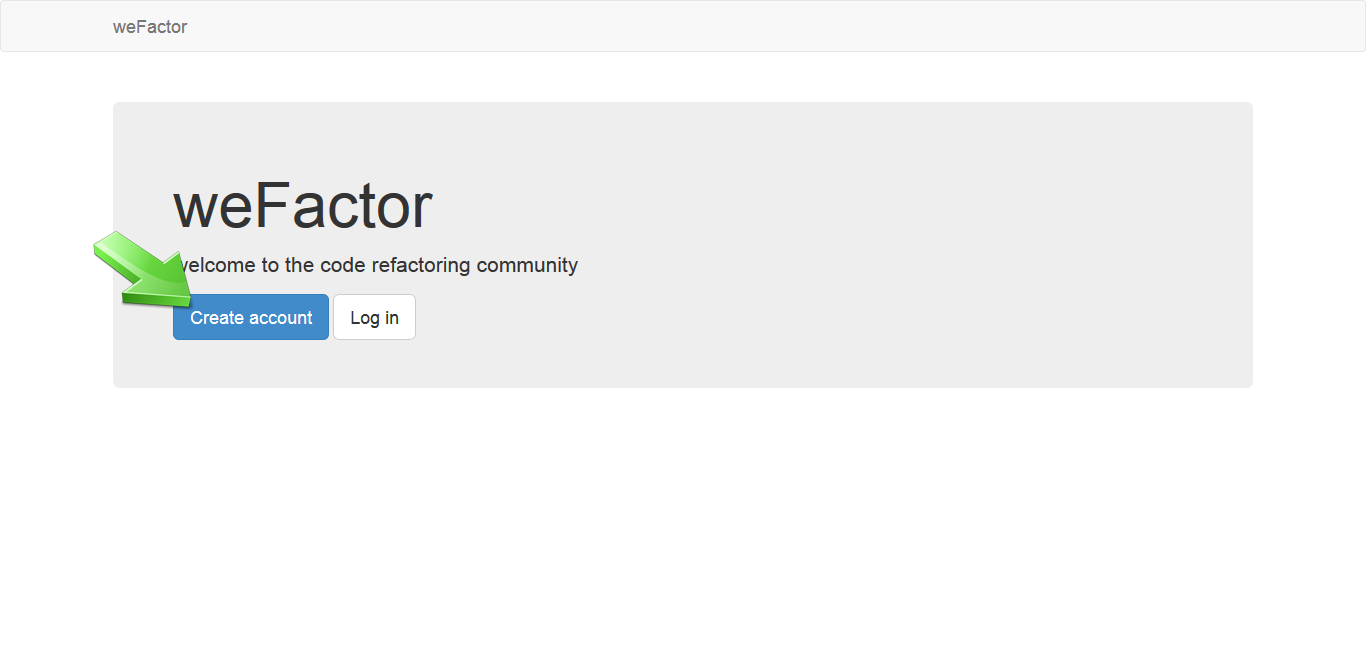
\includegraphics[width=0.8\textwidth]{Bilder/2.png}
    \caption{Accounterstellungsseite 1}
    \label{fig:accounterstellungsseite1}
\end{figure}


Wurde der Button geklickt gelangt man auf die gewünschte Seite.

\begin{figure}[H]
    \centering
    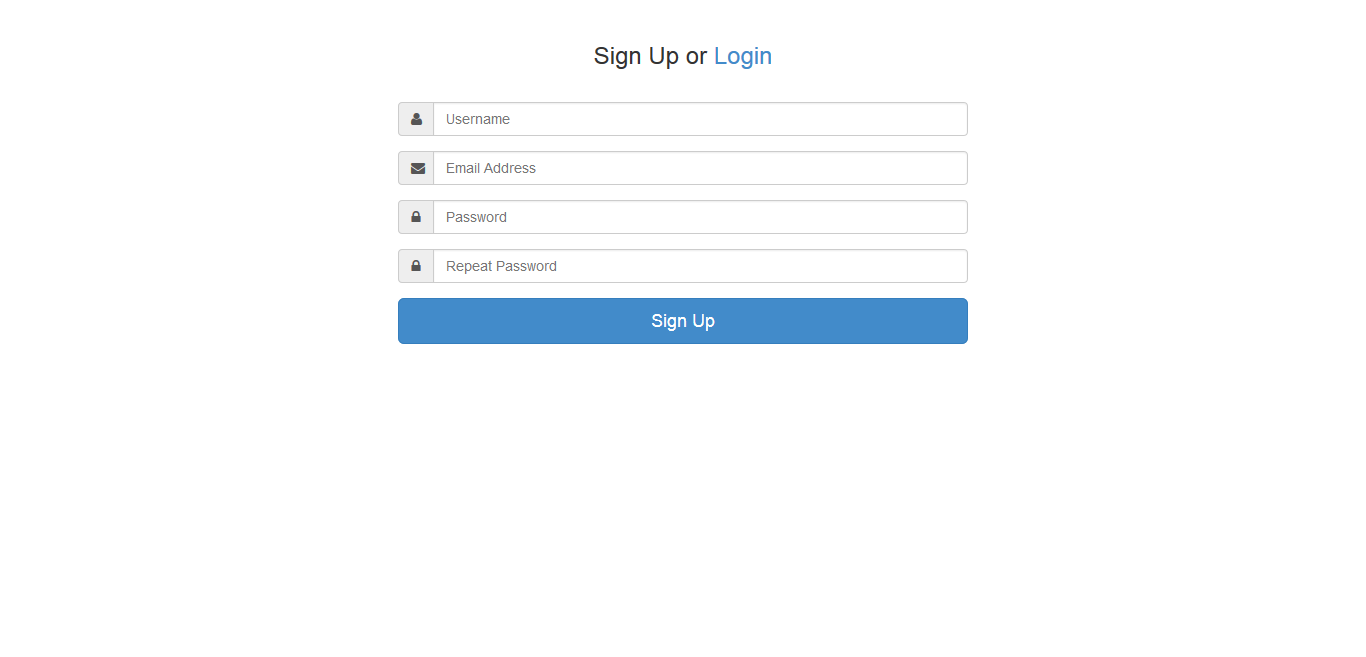
\includegraphics[width=0.8\textwidth]{Bilder/4.png}
    \caption{Accounterstellungsseite 2 }
    \label{fig:accounterstellungsseite2}
\end{figure}



Um seinen neuen Account erstellen zu können, müssen die jeweiligen Felder korrekt ausgefüllt werden.

\begin{figure}[H]
    \centering
    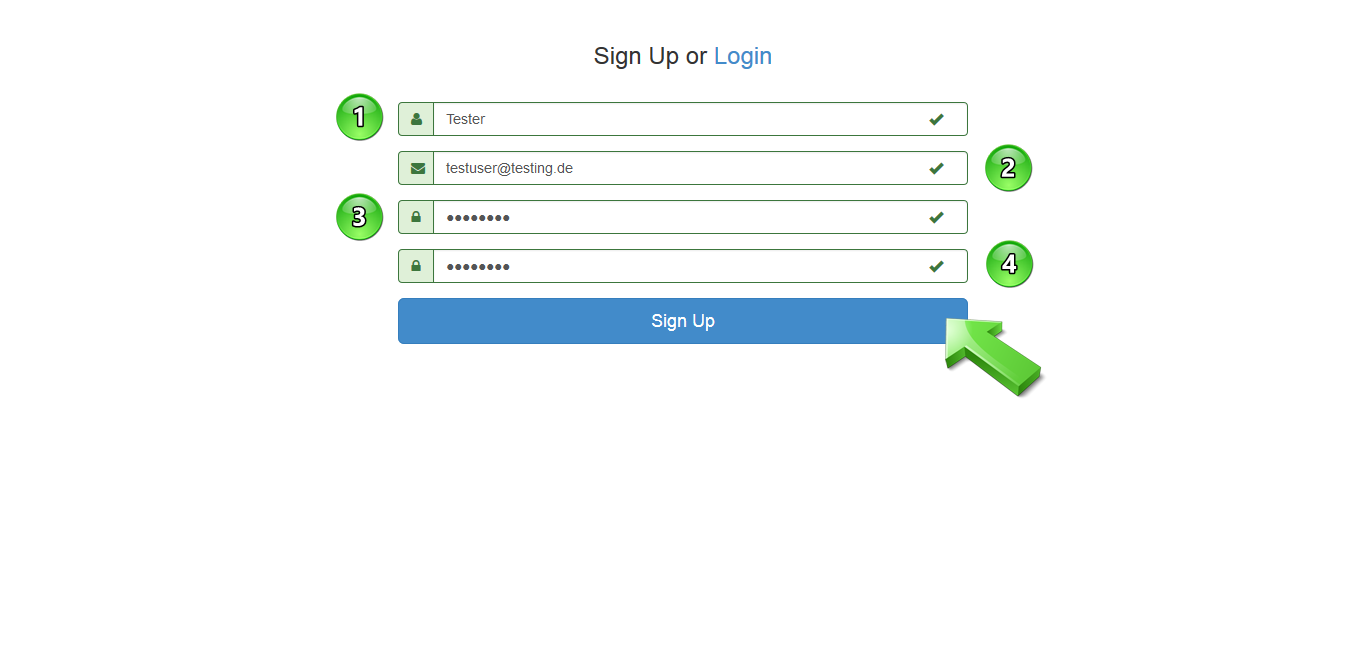
\includegraphics[width=0.8\textwidth]{Bilder/5.png}
    \caption{Accounterstellungsseite 3 }
    \label{fig:accounterstellungsseite3}
\end{figure}


\begin{enumerate}
\item Der Benutzername muss mindestens drei und darf höchstens 30 Zeichen lang sein.
\item Die Eingabe muss eine gültige E-Mail Adresse sein.
\item Das Passwort muss mindestens 8 und darf höchstens 30 Zeichen lang sein.
\item Die Passwortbestätigung muss mit dem zuvor eingegeben Passwort übereinstimmen.
\end{enumerate}

 
Werden in der Anwendung alle Felder grün umrahmt und ein Häkchen gesetzt, wurden alle Daten korrekt eingegeben und der „Sign Up“ Button kann ohne Fehlermeldung geklickt werden.
Durch das Klicken des Buttons wird der Account erstellt. Anschließend wird man auf die Startseite weitergeleitet.


\chapter{Login}
Um auf die Loginseite zu gelangen, wird auf den Button „Login“ geklickt.

\begin{figure}[H]
    \centering
    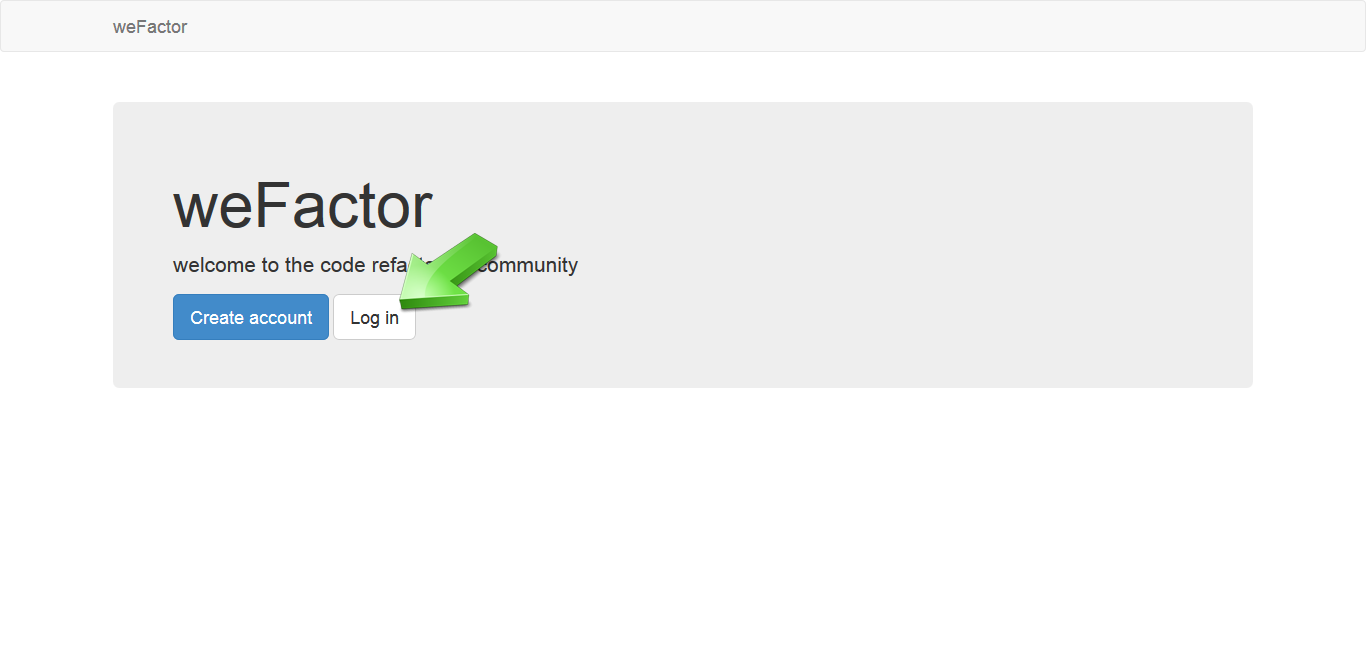
\includegraphics[width=0.8\textwidth]{Bilder/3.png}
    \caption{Loginseite 1 }
    \label{fig:loginseite1}
\end{figure}


Wurde der Button geklickt gelangt man auf die gewünschte Seite.

\begin{figure}[H]
    \centering
    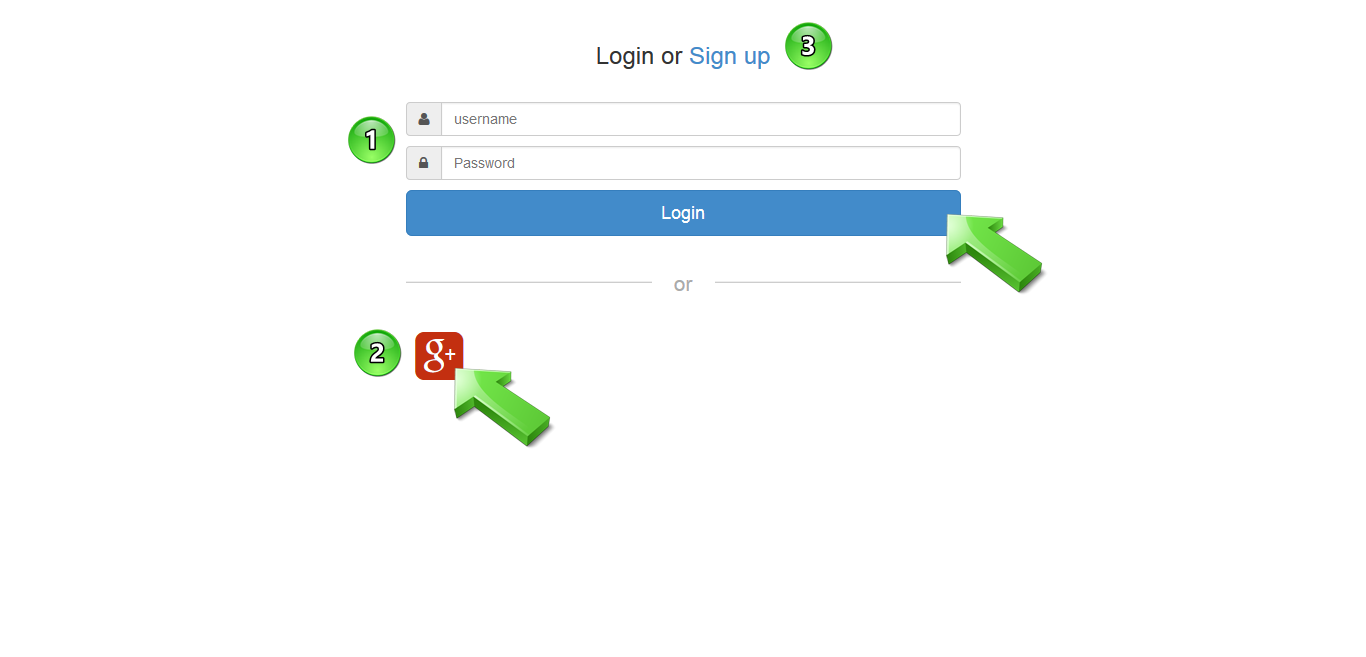
\includegraphics[width=0.8\textwidth]{Bilder/8.png}
    \caption{Loginseite 2 }
    \label{fig:loginseite2}
\end{figure}



Um sich einloggen zu können, müssen die jeweiligen Felder korrekt ausgefüllt werden. 
\begin{enumerate}
\item Benutzername und Passwort werden für einen erfolgreichen Login benötigt.
\item Um die Möglichkeit sich mit einem Google+ Account anzumelden, kann dieser Button geklickt werden.
\item Hat man sich doch entschieden einen neuen Account zu erstellen, kann auf „Sign Up“ die Seite wieder gewechselt werden.
\end{enumerate}


Entscheidet man sich, sich über Google+ einzuloggen wird man nach Klicken des Google+ Buttons direkt weitergeleitet.
Loggt man sich mit einem auf der Anwendung erstellten Accounts an, ist es nötig den „Login“ Button zu klicken um weitergeleitet zu werden.


\chapter{Startseite/Alle Funktionen im Schnelldurchlauf}

\begin{figure}[H]
    \centering
    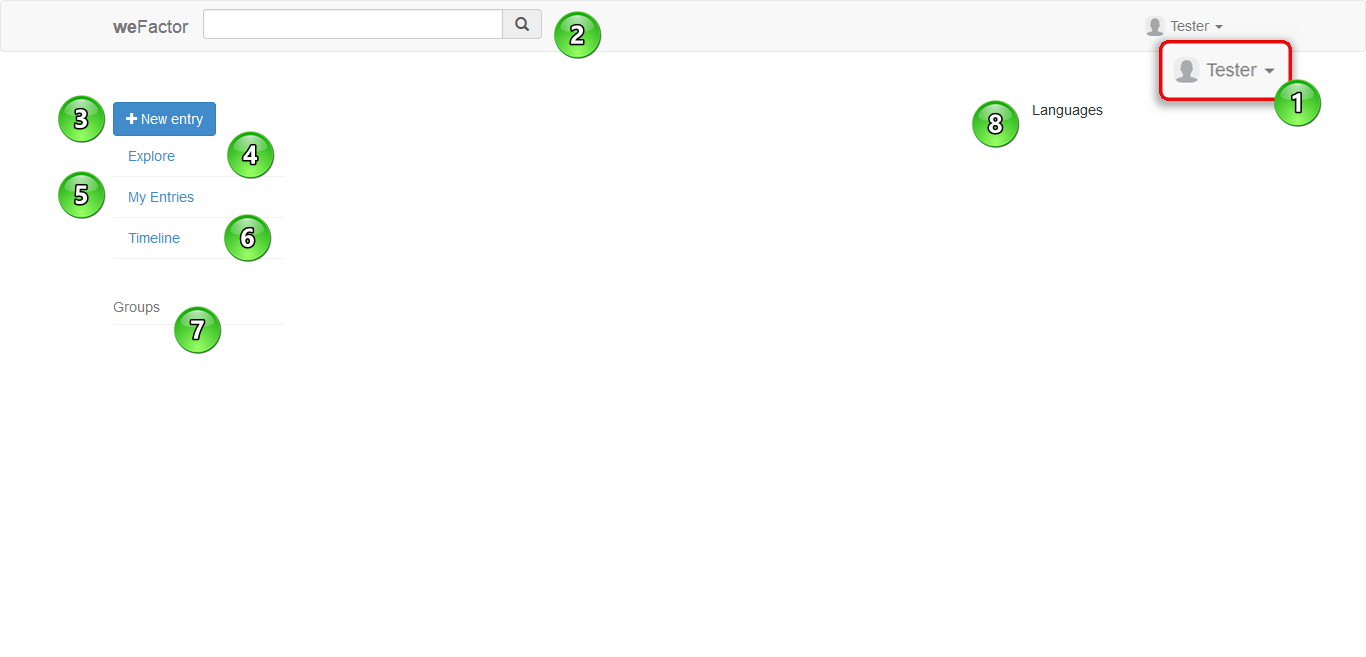
\includegraphics[width=0.8\textwidth]{Bilder/6.png}
    \caption{Exploreseite 1 }
    \label{fig:exploreseite1 }
\end{figure}



\begin{enumerate}
\item Anzeige des zurzeit angemeldeten Benutzers.
\item Suchfunktion: gesucht werden kann nach Benutzern, Tags, sowie Titel oder Beschreibung von Einträgen.
\item Auf „New Entry“ kann ein neuer Eintrag erstellt werden.
\item Auf „Explore“ werden alle Einträge der Anwendung nach Erstellungsdatum sortiert aufgelistet.
\item Auf „My Entries“ werden alle selbsterstellten Einträge nach Erstellungsdatum sortiert aufgelistet.
\item Auf „Timeline“ werden alle, den angemeldeten Benutzer betreffenden, Ereignisse nach Ereignisdatum sortiert aufgelistet.
\item Auf „Groups“ werden alle existierenden Gruppen der Anwendung aufgelistet. Zusätzlich gibt es eine Suchfunktion, sowie eine
\end{enumerate}

Filterfunktion für die Gruppe denen man beigetreten ist. Die schon beigetretenen Gruppen werden als Unterpunkte von „Groups“ angezeigt.


\begin{figure}[H]
    \centering
    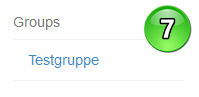
\includegraphics[width=0.25\textwidth]{Bilder/39.png}
    \caption{Großansicht Groups }
    \label{fig:grossansicht_groups}
\end{figure}


\chapter{Profileigenschaften und Logout}

Profileinstellungen und/oder ausloggen kann man sich, indem rechts oben auf den angemeldeten Benutzer geklickt wird und sich das Dropdownmenu öffnet.

\begin{figure}[H]
    \centering
    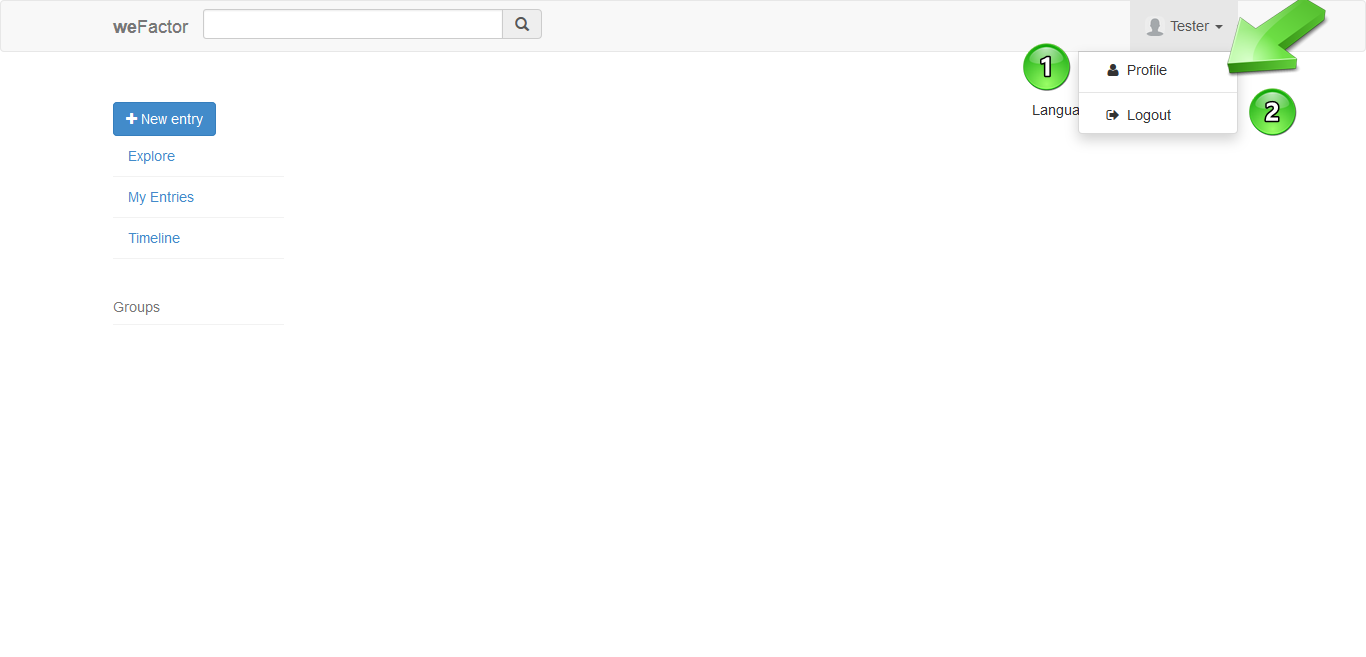
\includegraphics[width=0.8\textwidth]{Bilder/7.png}
    \caption{Benutzercombobox }
    \label{fig:beuntzercombobox}
\end{figure}



\begin{enumerate}
\item Wird auf „Logout“ geklickt, wird man ausgeloggt und auf die Loginseite weitergeleitet.
\item „Profile“ leitet an die Profileigenschaftenseite weiter. Hier können alle Daten zum jeweiligen Benutzer eingesehen werden.
\end{enumerate}




\chapter{Profileigenschaften ändern}
Wird im gerade erwähnten Dropdownmenu „Profile“ ausgewählt, wird man auf die Profileigenschaftenseite weitergeleitet.

\begin{figure}[H]
    \centering
    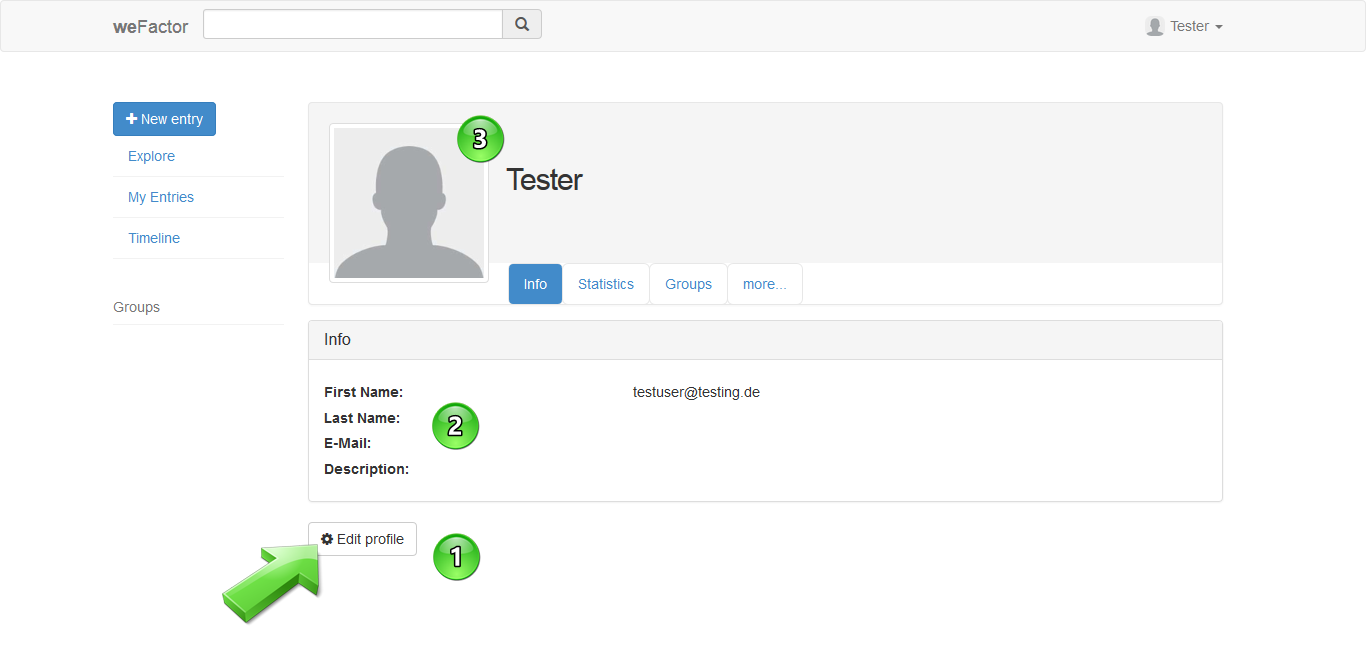
\includegraphics[width=0.8\textwidth]{Bilder/9.png}
    \caption{Profilbearbeitungsseite 1}
    \label{fig:profilbearbeitungsseite1}
\end{figure}


\begin{enumerate}
\item Weiterleitung zur nächsten Seite, um Profileigenschaften erweitern oder gegebenenfalls ändern zu können.
\item Infos zum jeweiligen Benutzer, welche geändert werden können.
\item Profilfoto des Benutzers. Wird über Google+ eingeloggt, so wird eben diese Profilfoto auch auf der Anwendung angezeigt.
\end{enumerate}


Wird auf den Button „Edit profile“ geklickt, können die jeweiligen Eigenschaften neu ausgefüllt werden.

\begin{figure}[H]
    \centering
    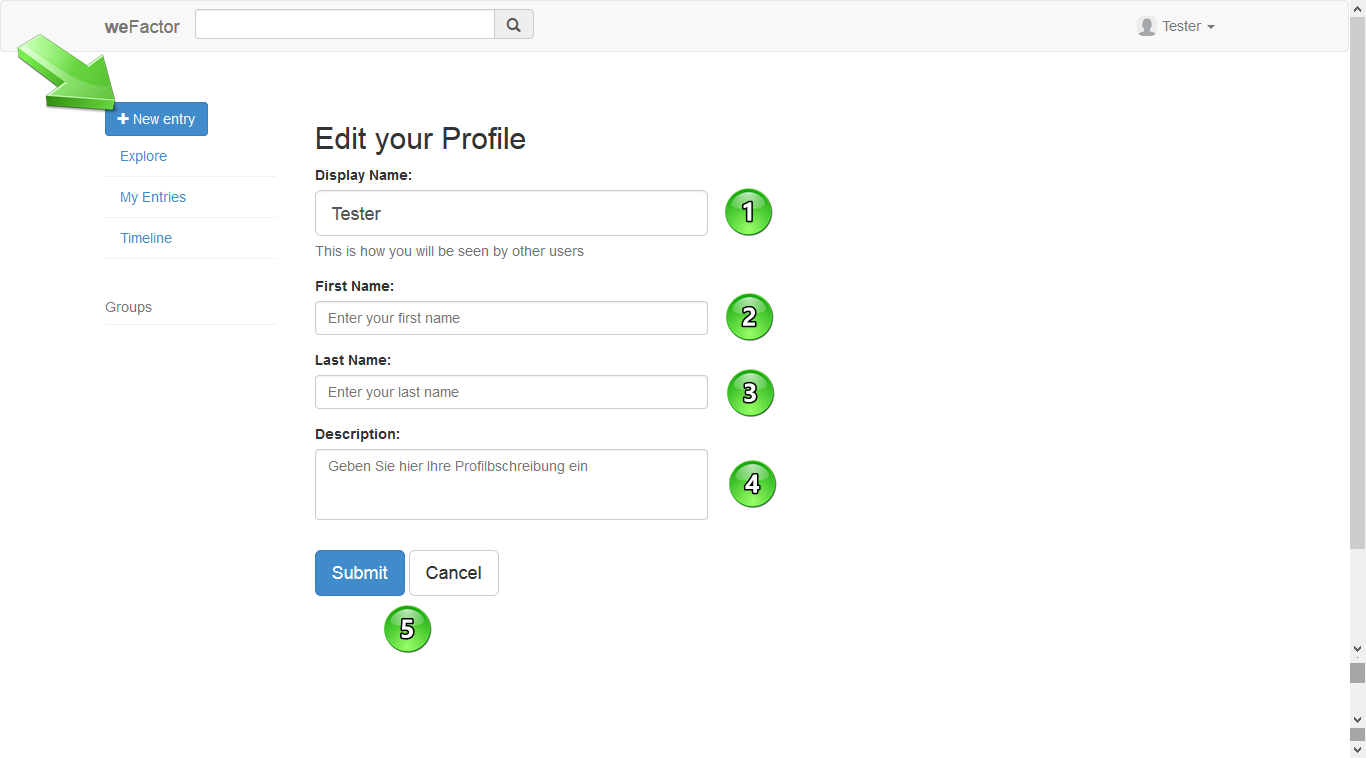
\includegraphics[width=0.8\textwidth]{Bilder/10.png}
    \caption{Profilbearbeitungsseite 2 }
    \label{fig:profilbearbeitungsseite2}
\end{figure}


\begin{enumerate}
\item Der Name, mit dem man für andere Benutzer angezeigt wird.
\item Der Vorname des Benutzers.
\item Der Nachname des Benutzers.
\item Die Beschreibung, um gegebenenfalls noch mehr Information preiszugeben.
\item Möglichkeit das Geänderte auf „Submit“ zu speichern, oder auf „Cancel“ zu verwerfen.
\end{enumerate}


Als nächsten Schritt wird ein neuer Eintrag erstellt.


\chapter{New Entry, einen neuen Eintrag erstellen/ändern/löschen}

Wird in der Navigationsbar links auf „New Entry“ geklickt, wird man auf die Eintragserstellungsseite weitergeleitet.

\begin{figure}[H]
    \centering
    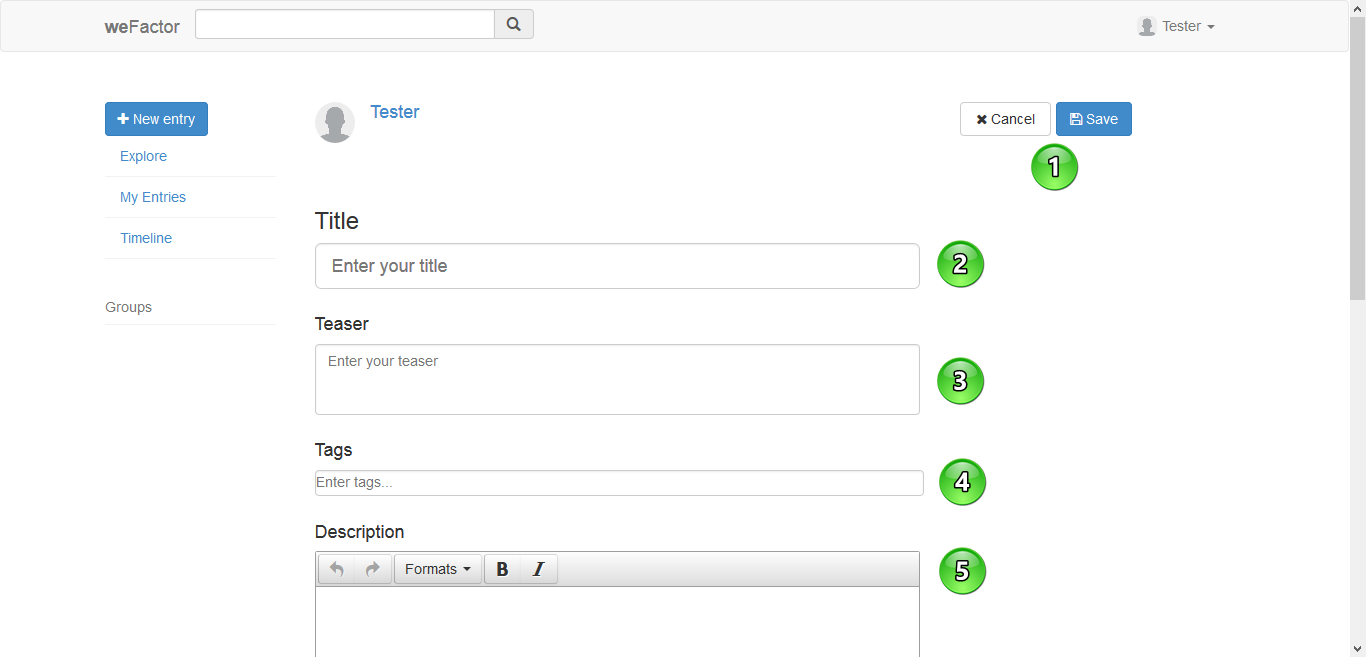
\includegraphics[width=0.8\textwidth]{Bilder/11.png}
    \caption{Eintragerstellungsseite 1 }
    \label{fig:eintragerstellungsseite1}
\end{figure}
\begin{figure}[H]
    \centering
    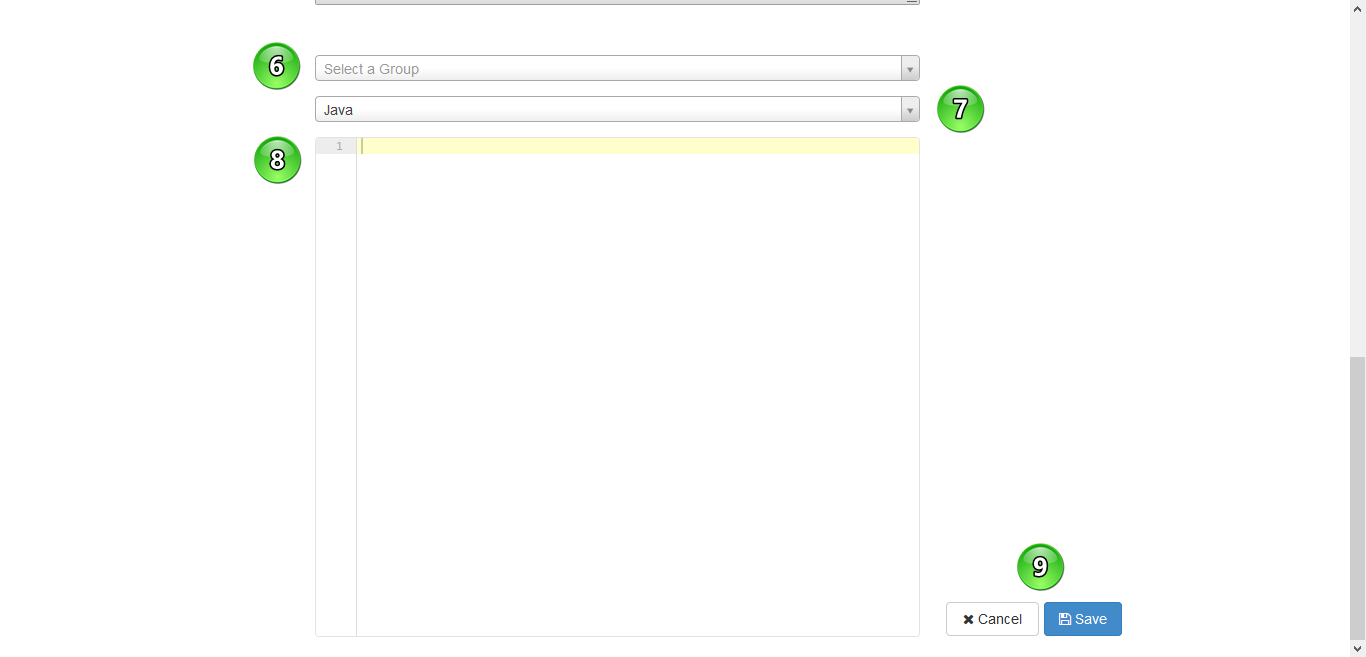
\includegraphics[width=0.8\textwidth]{Bilder/12.png}
    \caption{Eintragerstellungsseite 2 }
    \label{fig:eintragerstellungsseite2}
\end{figure}


\begin{enumerate}
\item Möglichkeit das Eingegebene auf „Save“ zu speichern, oder auf „Cancel“ zu verwerfen.
\item Titel des Eintrages.
\item Teaser des Eintrages, um andere Mitglieder der Anwendung auf den Eintrag aufmerksam zu machen.
\item Den Eintrag mit Tags versehen, damit dieser einfacher gefunden werden kann.
\item Beschreibung, um den Programm-Code des Eintrages besser erläutern zu können.
\item Eine der beigetretenen Gruppen auswählen, damit dieser Eintrag nur von Benutzern in der jeweilig ausgewählten Gruppe angesehen werden kann.


\begin{figure}[H]
    \centering
    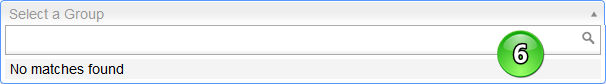
\includegraphics[width=0.8\textwidth]{Bilder/13.png}
    \caption{Eintragsgruppenauswahl }
    \label{fig:eintragsgruppenauswahl}
\end{figure}



\item Sprache auswählen, in der Programm-Code, in diesem Eintrag verfasst wurde.

\begin{figure}[H]
    \centering
    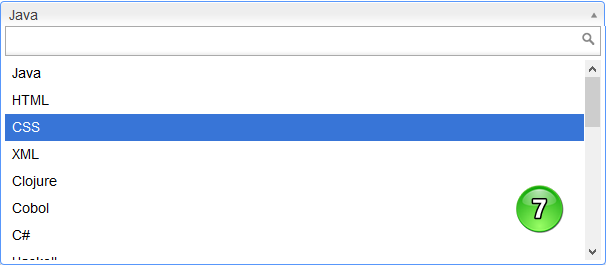
\includegraphics[width=0.8\textwidth]{Bilder/14.png}
    \caption{Eintragsprogrammiersprachenauswahl }
    \label{fig:eintragsprogrammiersprachenauswahl}
\end{figure}




\item Editor in dem der Programm-Code geschrieben werden kann. 
\item Möglichkeit das Eingegebene auf „Save“ zu speichern, oder auf „Cancel“ zu verwerfen.
\end{enumerate}


Wird nun auf den Button „Save“ geklickt, wird man auf Eintragsübersichtseite weitergeleitet.

\begin{figure}[H]
    \centering
    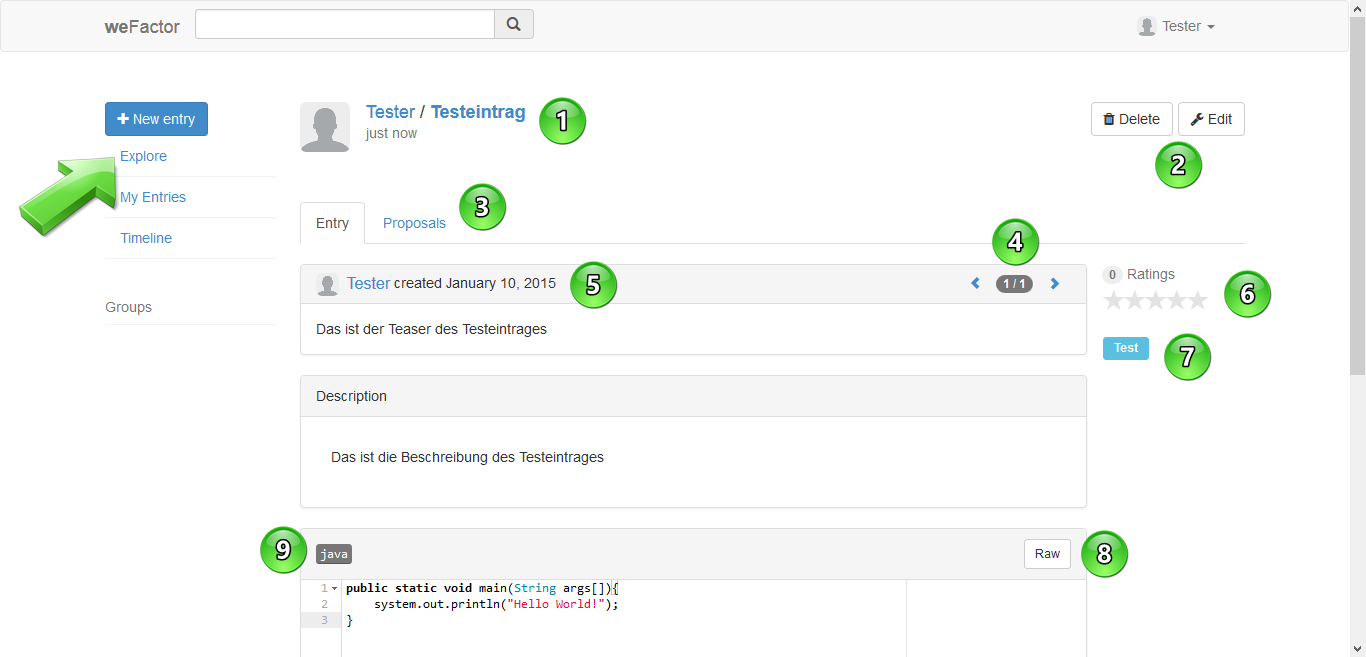
\includegraphics[width=0.8\textwidth]{Bilder/15.png}
    \caption{Eintragsuebersichtsseite 1 }
    \label{fig:eintragsuebersichtsseite1}
\end{figure}



\begin{enumerate}
\item Name des Benutzers/ Name des Eintrags, sowie der Erstellungszeitpunkt.
\item Möglichkeit den Eintrag auf „Edit“ zu bearbeiten, oder auf „Delete“ zu löschen.
\item Beim Reiter „Entry“ die Eintragsübersicht anzeigen lassen und beim Reiter „Proposals“ die Vorschläge andere Mitglieder für diesen Eintrag einsehen.
\item Wurden weitere Vorschläge für diesen Eintrag erstellt, kann man zwischen diesen durchwechseln.
\item Für jeden dieser Vorschläge wird angezeigt, wann und von wem der jeweilige Vorschlag erstellt wurde.
\item Einträge und Vorschläge können auf einer Sterneskala von eins bis fünf bewertet werden.
\item Tags unter denen der Eintrag oder Vorschlag gefunden werden kann.
\item Den Button „Raw“ klicken um auf eine Seite weitergeleitet zu werden, welche nur den Programm-Code anzeigt. Dieser kann dann in die Zwischenablage kopiert werden.
\item Programmiersprache in der der Programm-Code geschrieben wurde.
\end{enumerate}



Nach Erstellung des ersten Eintrages zu „Explore“ wechseln.


\chapter{Explore, alle Einträge in der Anwendung einsehen}

Wird links in der Navigationsbar auf „Explore“ geklickt, werden alle Einträge in der Anwendung nach Erstellungsdatum aufgelistet. Die Auflistung kann durch dich Suchfunktion, sowie der Filterung(welche in Kapitel erläutert wird) auf genauere Ergebnisse begrenzt werden.

\begin{figure}[H]
    \centering
    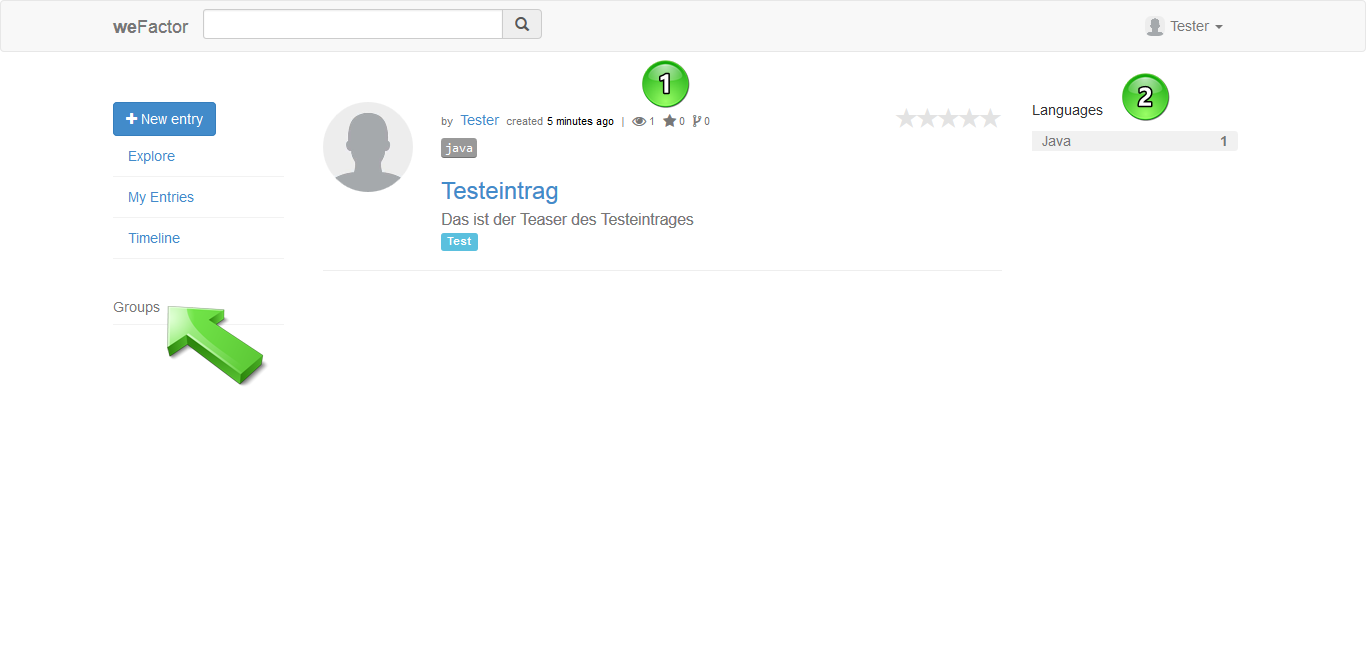
\includegraphics[width=0.8\textwidth]{Bilder/16.png}
    \caption{Exploreseite 2 }
    \label{fig:exploreseite2}
\end{figure}



\begin{enumerate}
\item Die drei Icons haben folgende Bedeutung:
\begin{enumerate}
\item Das kleine Auge zeigt an, wie oft des Eintrages angeschaut wurde.
\item Der kleine Stern zeigt an, wie oft der Eintrag bewertet wurde.
\item Der kleine Zweig zeigt an, wie viele Vorschläge es für diesen Eintrag gibt.
\end{enumerate}
\item Anzeige wie viele Einträge es in der Anwendung in den jeweiligen Programmiersprachen gibt.

\end{enumerate}


Als nächsten Schritt wird eine neue Gruppe erstellt.


\chapter{Groups, eine/r neue Gruppe erstellen/beitreten/verlassen}

Wird links in der Navigationsbar auf „Groups“ geklickt, werden alle Gruppen denen man beigetreten ist, aufgelistet.

\begin{figure}[H]
    \centering
    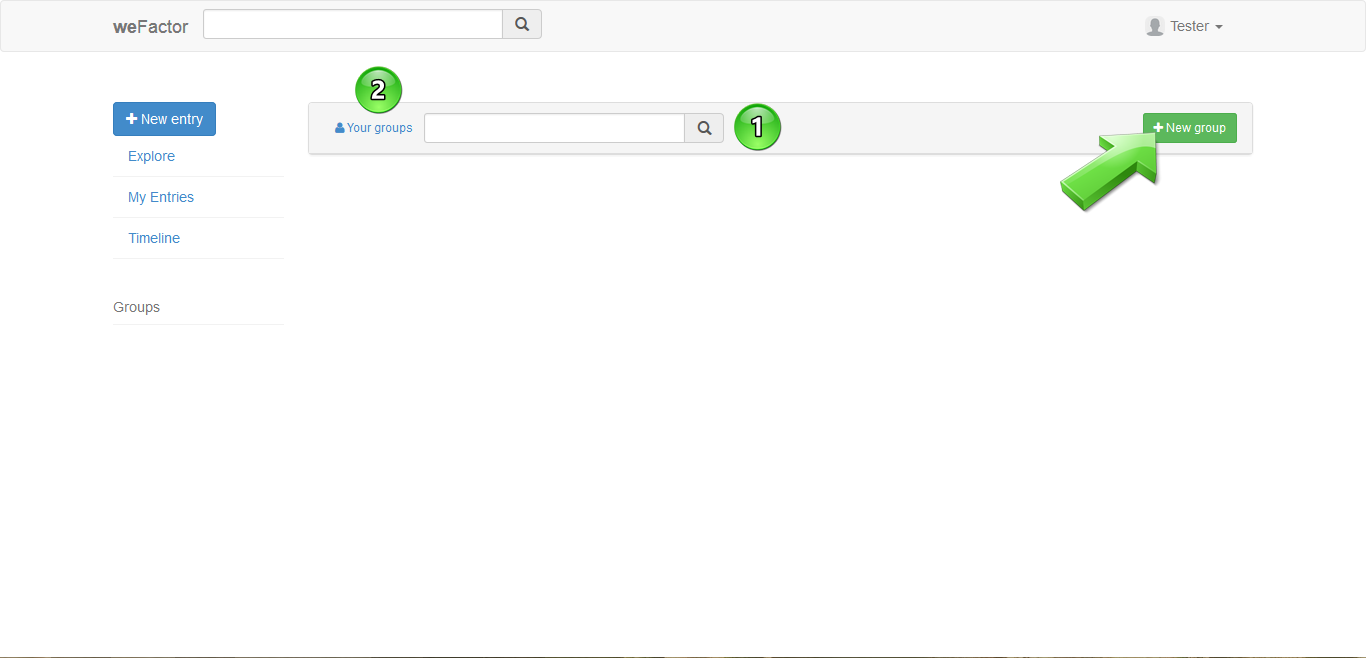
\includegraphics[width=0.8\textwidth]{Bilder/17.png}
    \caption{Gruppenauswahlseite 1 }
    \label{fig:gruppenauswahlseite 1}
\end{figure}


\begin{enumerate}
\item Eine Suchfunktion speziell für Gruppen.
\item Schnelle Filterungsfunktion, um nur Gruppen anzeigen zu lassen, denen der Benutzer beigetreten ist.

\end{enumerate}


Um eine neue Gruppe zu erstellen, wird auf den Button „New Group“ geklickt.

\begin{figure}[H]
    \centering
    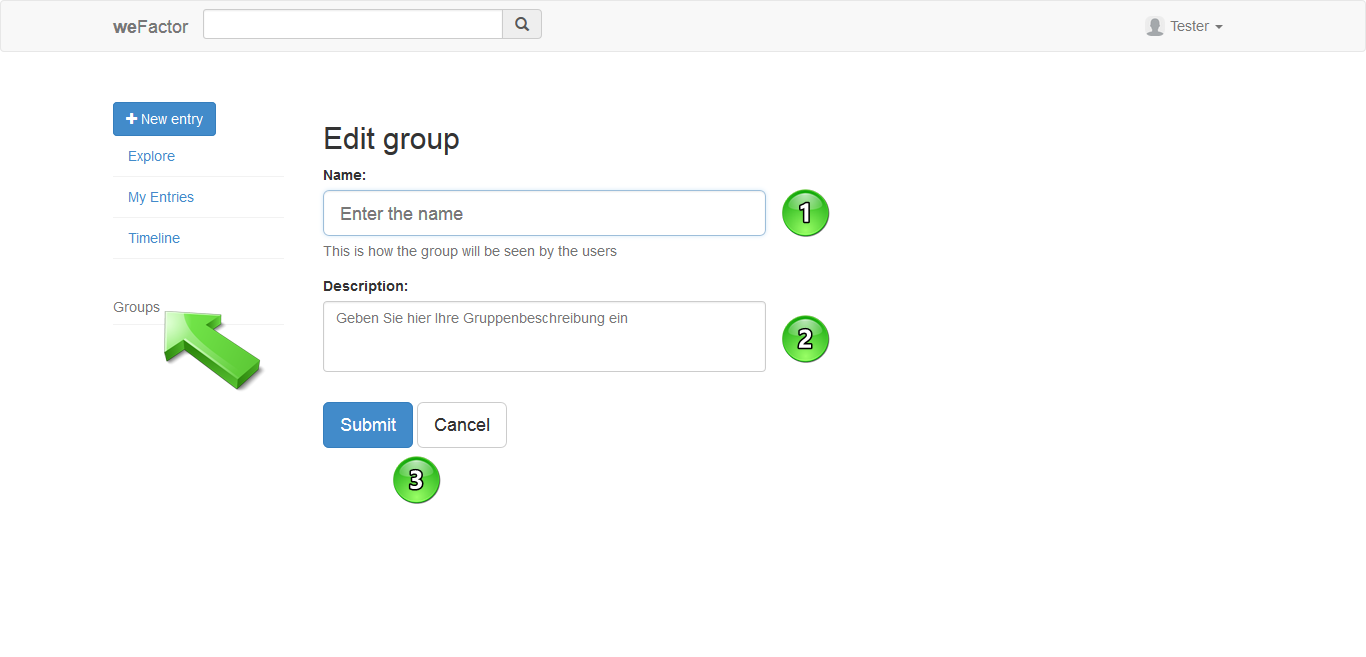
\includegraphics[width=0.8\textwidth]{Bilder/18.png}
    \caption{Gruppenerstellungsseite }
    \label{fig:gruppenerstellungsseite}
\end{figure}


Um die Erstellung abzuschließen, muss einen Name und eine Beschreibung eingegeben werden.

\begin{enumerate}
\item Der Gruppenname muss mindestens drei und darf höchstens 50 Zeichen lang sein.
\item Die Gruppenbeschreibung muss mindestens zehn und darf höchstens 300 Zeichen lang sein.
\item Möglichkeit die Gruppe auf „Submit“ zu erstellen, oder auf „Cancel“ zu verwerfen.
\end{enumerate}


Wird jetzt in der Navigationsbar wieder auf „Groups“ geklickt, erscheint in der Gruppenübersicht die gerade erstellte Gruppe.

\begin{figure}[H]
    \centering
    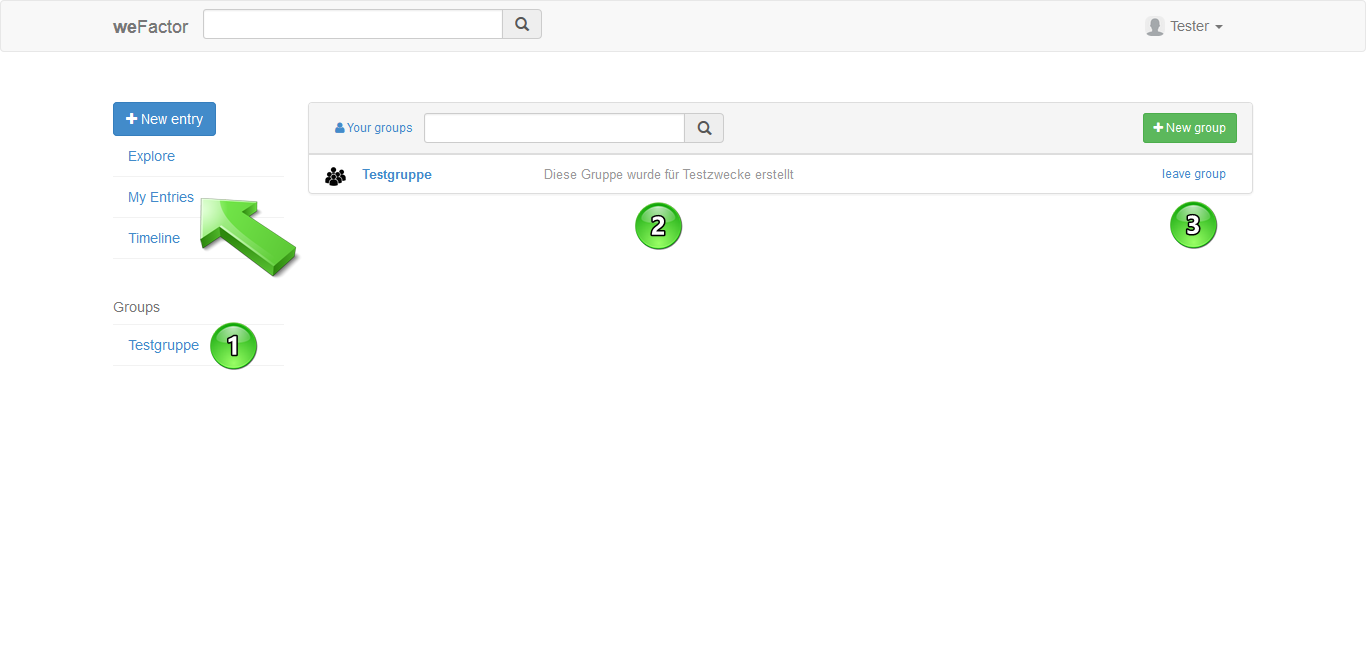
\includegraphics[width=0.8\textwidth]{Bilder/19.png}
    \caption{Gruppenauswahlseite 2}
    \label{fig:gruppenauswahlseite2}
\end{figure}



\begin{enumerate}
\item Gruppen, denen der Benutzer beigetreten ist, werden in der Navigationsbar als Untergruppen von „Groups“ aufgelistet.
\item Die Beschreibung der Gruppe.
\item Die Möglichkeit, die Gruppe wieder zu verlassen.
\end{enumerate}


Als nächsten Schritt alle Einträge, die vom Benutzer erstellt wurde, anzeigen lassen.


\chapter{My Entries, alle vom Benutzer erstellten Einträge}

Wird links in der Navigationsbar auf „My Entries“ geklickt, werden alle Einträge nach Erstellungsdatum aufgelistet, die der angemeldete Benutzer erstellt hat.

\begin{figure}[H]
    \centering
    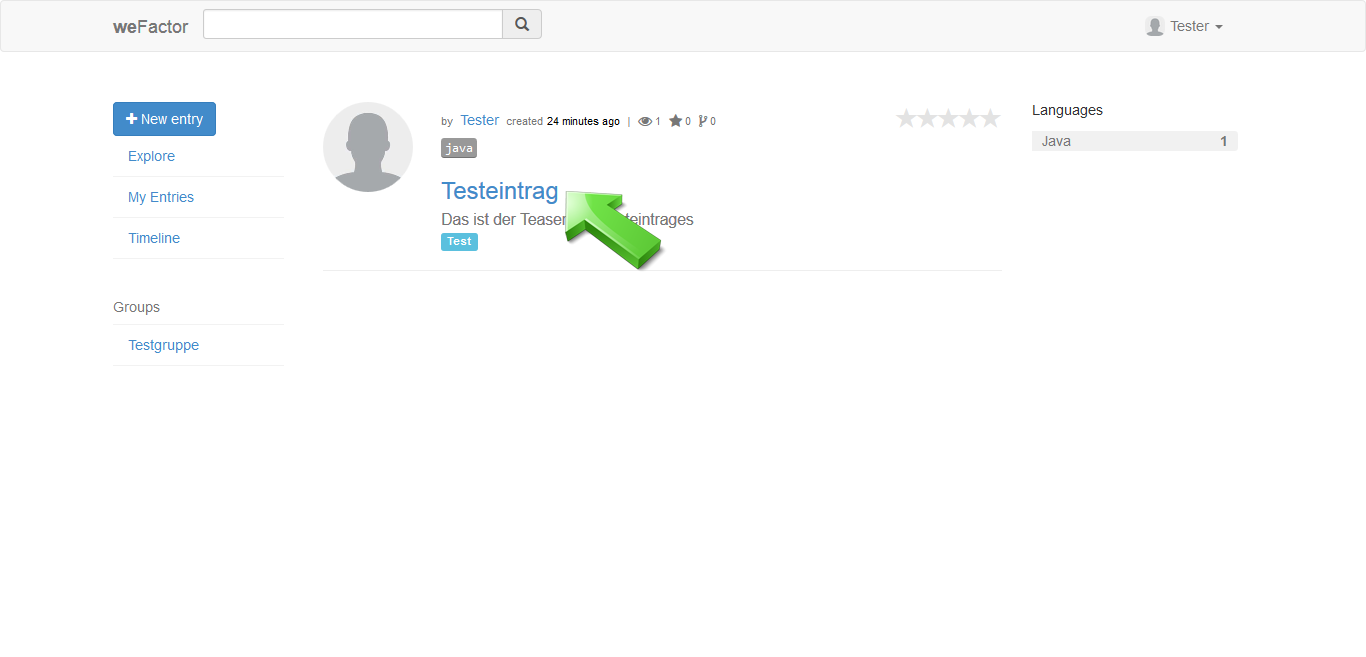
\includegraphics[width=0.8\textwidth]{Bilder/20.png}
    \caption{Exploreseite 3}
    \label{fig:exploreseite3}
\end{figure}


Als nächsten Schritt wird der Testeintrag in die erstellte Testgruppe verschoben.



\chapter{Einträge in eine andere Gruppe verschieben}

Wird auf den erstellten Testeintrag geklickt, wird dessen Eintragsübersichtsseite angezeigt.

\begin{figure}[H]
    \centering
    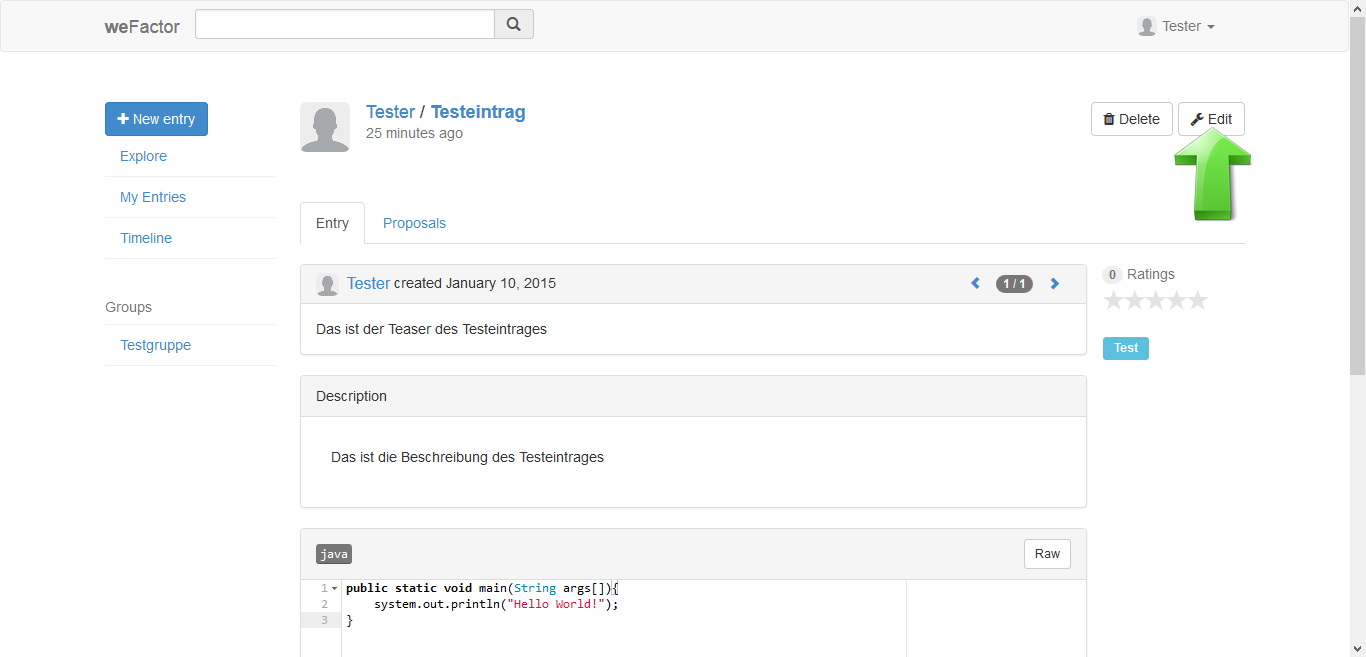
\includegraphics[width=0.8\textwidth]{Bilder/21.png}
    \caption{Eintraguebersichtsseite 2}
    \label{fig:eintraguebersichtsseite2}
\end{figure}


Wird auf den Button „Edit“ geklickt, wird man auf die Eintragsbearbeitungsseite weitergeleitet.

\begin{figure}[H]
    \centering
    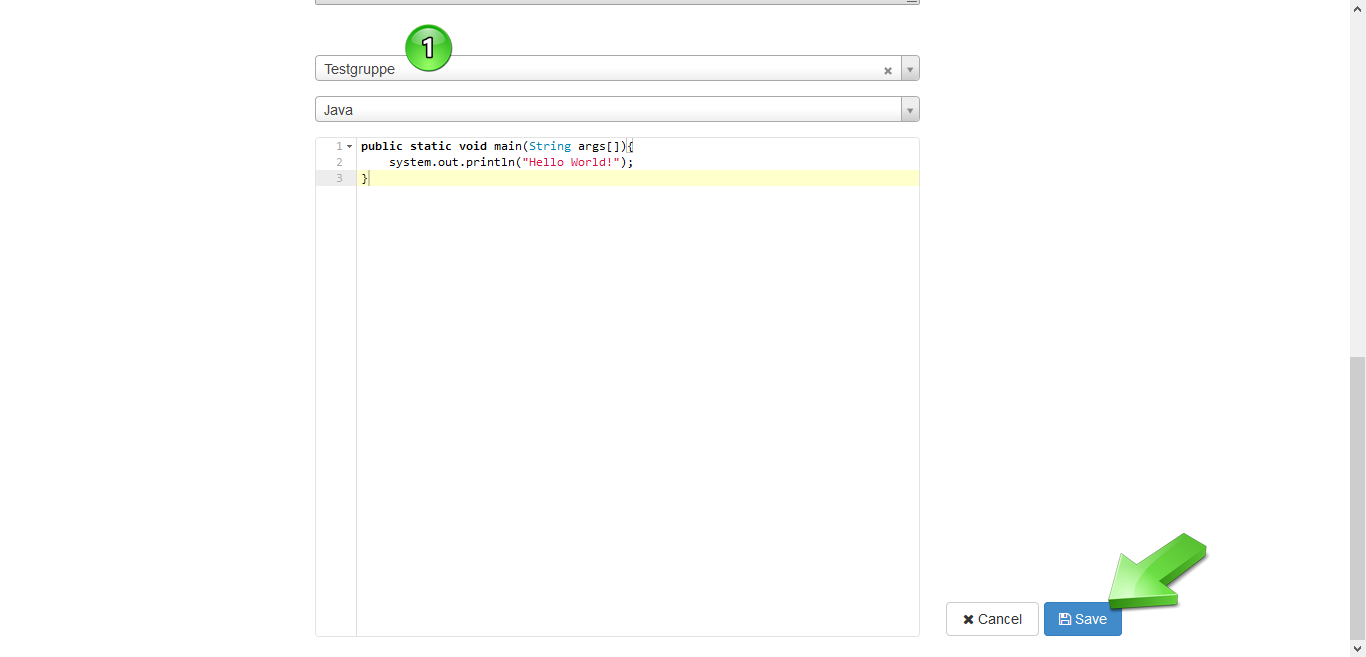
\includegraphics[width=0.8\textwidth]{Bilder/22.png}
    \caption{Eintragbearbeitungsseite}
    \label{fig:eintragbearbeitungsseite}
\end{figure}


\begin{enumerate}
\item Im Dropdownmenu „Select a Group“ kann nun die erstellte Testgruppe angegeben werden.
\end{enumerate}


Wird auf den Button „Save“ geklickt, wird die änderung gespeichert und man wird auf die Eintragsübersichtsseite weitergeleitet.
Als nächsten Schritt wird in der Navigationsbar links die Testgruppe aufgerufen.

\begin{figure}[H]
    \centering
    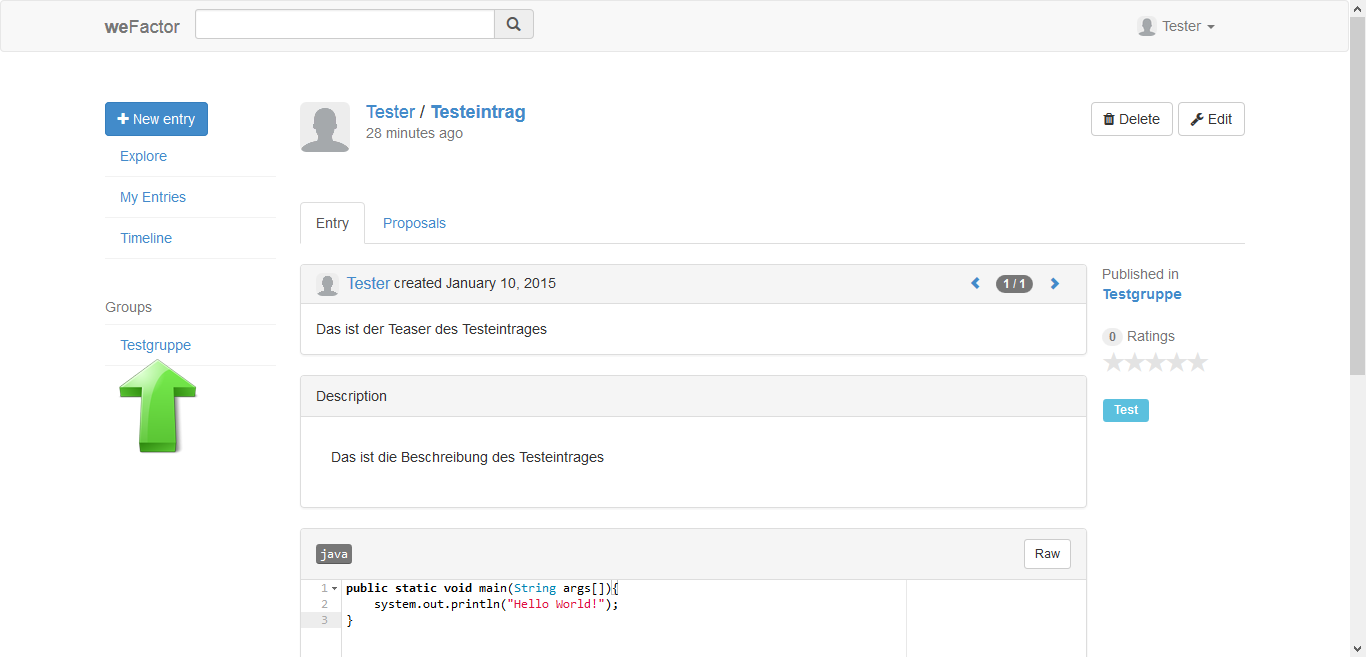
\includegraphics[width=0.8\textwidth]{Bilder/23.png}
    \caption{Eintraguebersichtsseite 3}
    \label{fig:eintraguebersichtsseite3}
\end{figure}


Danach wird übersicht der Testgruppe aufgerufen.

\begin{figure}[H]
    \centering
    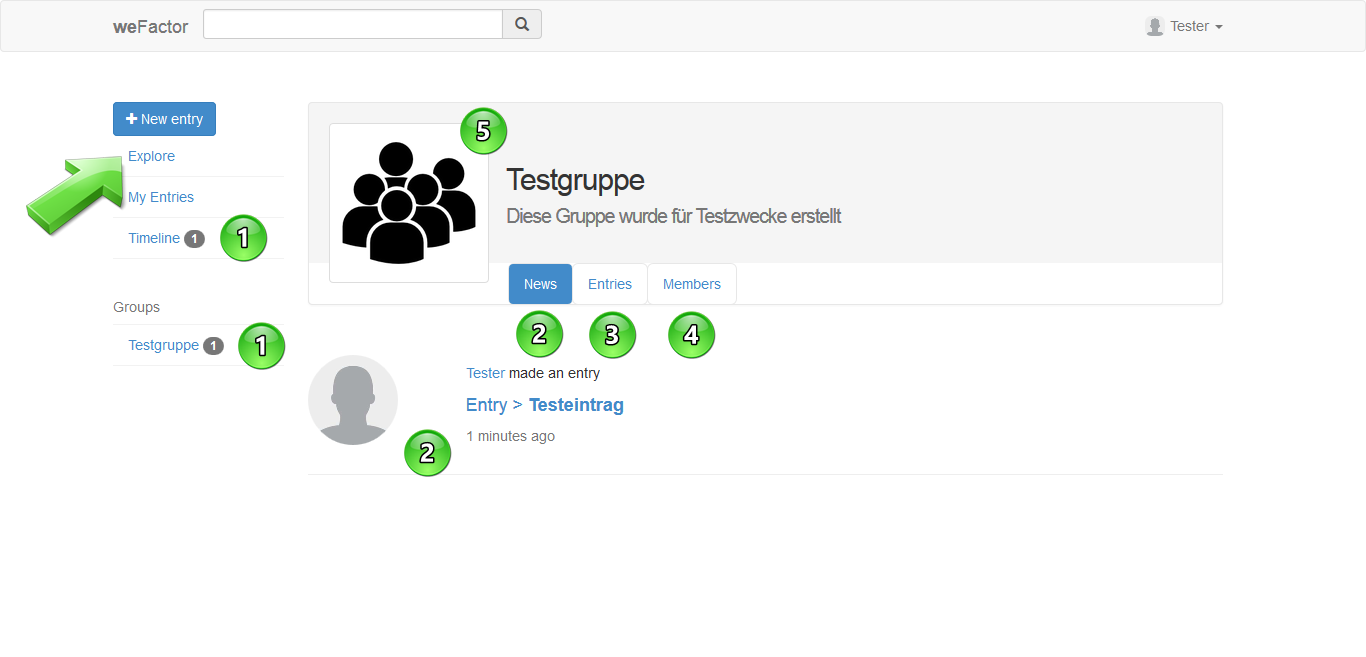
\includegraphics[width=0.8\textwidth]{Bilder/24.png}
    \caption{Gruppenuebersichtsseite}
    \label{fig:gruppenuebersichtsseite}
\end{figure}


\begin{enumerate}
\item Gibt es eine des Benutzer betreffende Neuigkeit, wird diese jedes Mal in der Timeline angezeigt und sowie hier auch in der betreffenden Gruppe. Dargestellt als eine Zahl, entsprechend der Menge an Neuigkeiten.
\item Da dem Testeintrag in den dessen Details die Testgruppe hinzugefügt wurde, wird dieser Eintrag jetzt nur noch in der Testgruppe angezeigt und für Mitglieder die dieser Gruppe nicht angehören nicht mehr einsehbar. Da die Verschiebung des Eintrages eine Neuigkeit in der Gruppe ist, wird dies im Reiter „News“ angezeigt.
\item Hier werden alle Einträge nach Erstellungsdatum sortiert aufgelistet, welche in der Gruppe eingestellt wurden.
\item Hier werden alle Mitglieder dieser Gruppe angezeigt.
\end{enumerate}


Als nächsten Schritt wird auf der „Explore“-Seite die Filterfunktion gezeigt.



\chapter{Suchfunktion mit/ohne Filter}

\begin{figure}[H]
    \centering
    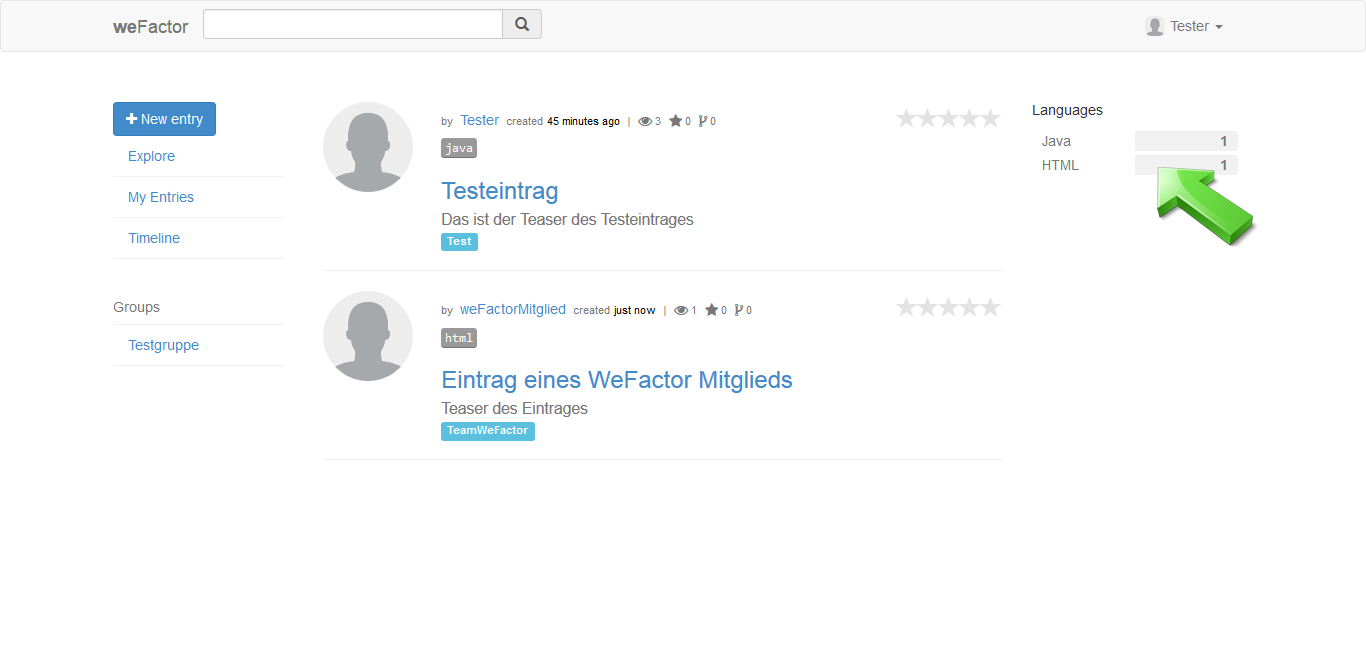
\includegraphics[width=0.8\textwidth]{Bilder/26.png}
    \caption{Sprachenfilterung 1}
    \label{fig:sprachenfilterung1}
\end{figure}


Auf der „Explore“-Seite wir rechts oben auf bei „Languages“ auf die Programmiersprache HTML geklickt.

\begin{figure}[H]
    \centering
    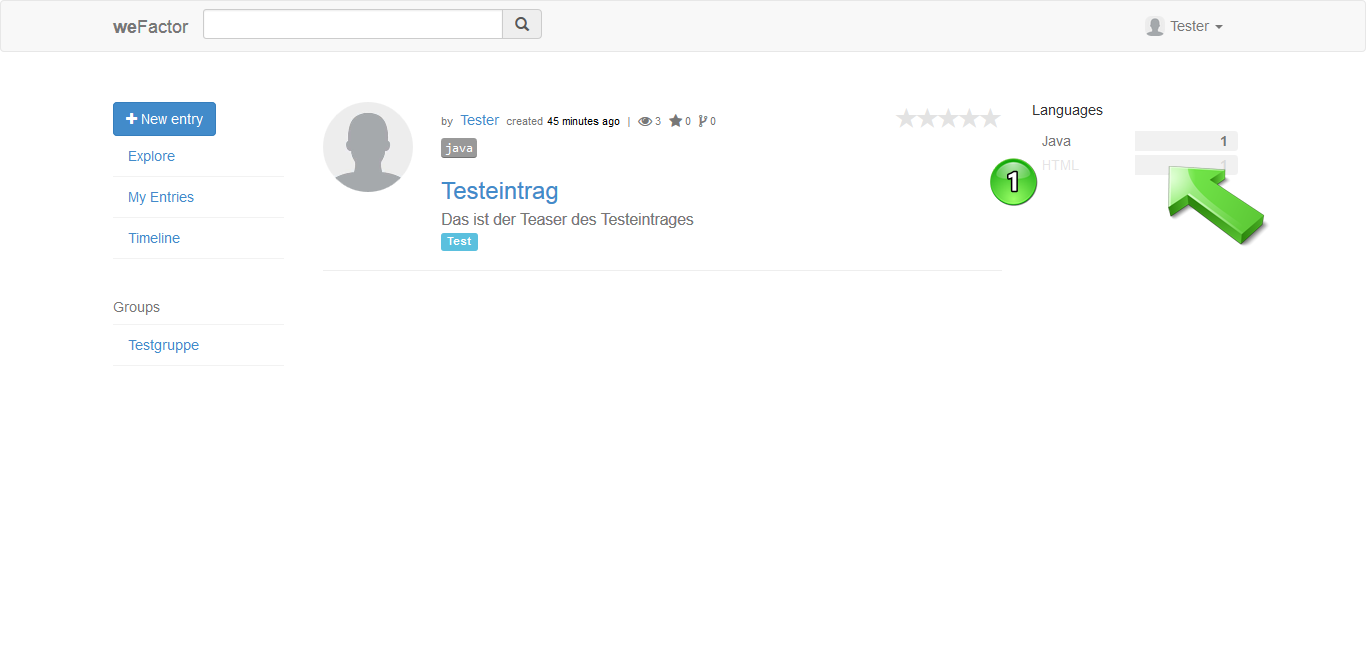
\includegraphics[width=0.8\textwidth]{Bilder/27.png}
    \caption{Sprachenfilterung 2}
    \label{fig:sprachenfilterung2}
\end{figure}


\begin{enumerate}
\item Wird auf eine oder mehrere der Sprachen geklickt, werden diese ausgegraut. Das bedeutet, dass diese bei Anzeige der Einträge nicht mehr berücksichtigt werden.
\end{enumerate}


Danach wird wieder auf HTML geklickt, um die Filterung rückgängig zu machen.
Als nächsten Schritt wird ein Vorschlag für einen Eintrag eines anderen Mitglieds erstellt.


 
\chapter{Proposals, Vorschläge für Einträge}
\section{Einen Vorschlag erstellen}
Um einen Vorschlag zu erstellen wird auf einen beliebigen Eintrag eines anderen Mitglieds geklickt.

\begin{figure}[H]
    \centering
    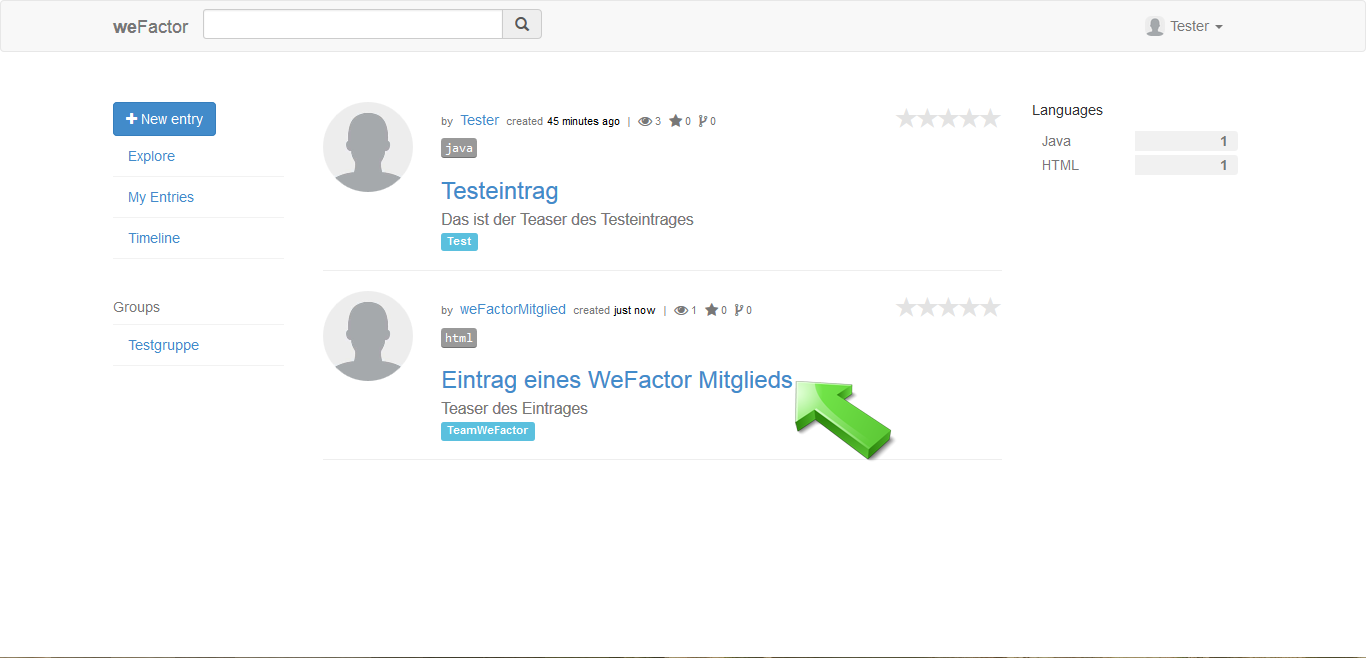
\includegraphics[width=0.8\textwidth]{Bilder/28.png}
    \caption{Mitgliedseintrag}
    \label{fig:Mitgliedseintrag}
\end{figure}


Auf der Eintragsübersicht klickt man nun auf „New Version“.

\begin{figure}[H]
    \centering
    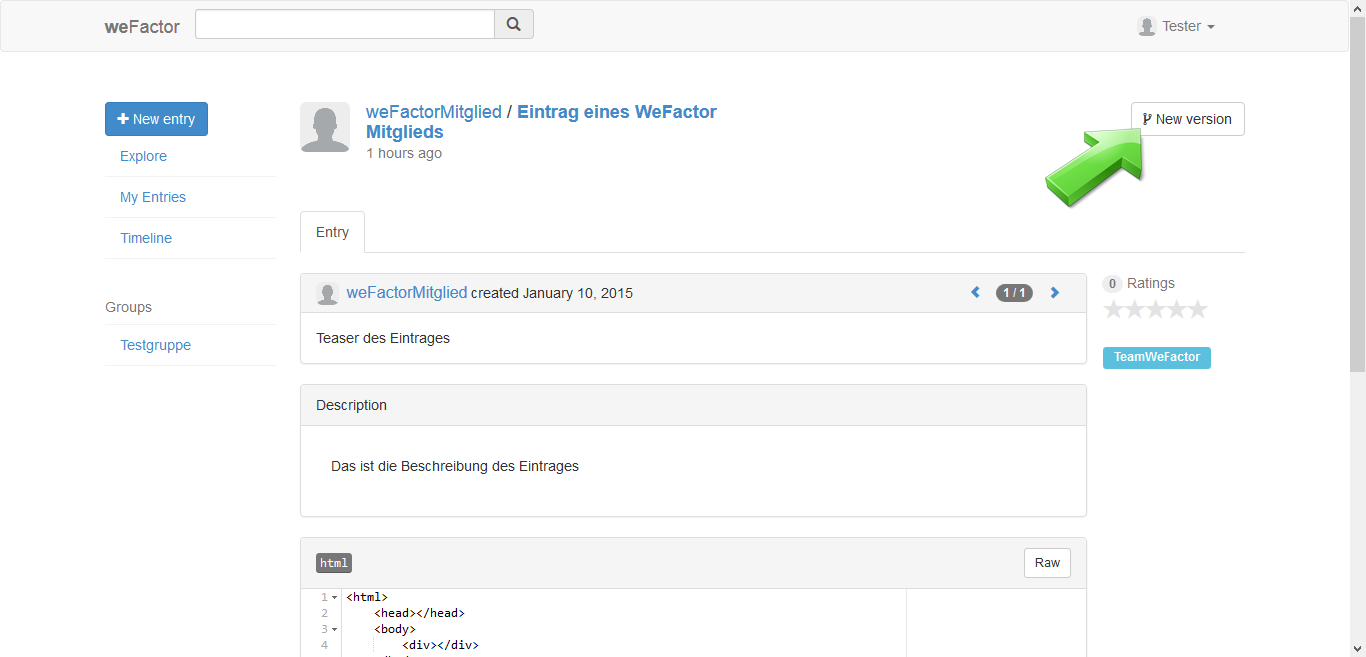
\includegraphics[width=0.8\textwidth]{Bilder/29.png}
    \caption{Versionserstellung 1}
    \label{fig:versionserstellung1}
\end{figure}


Um einen neuen Vorschlag zu erstellen, muss es eine möglichst sinnvolle änderung geben. Beispielsweise eine Verbesserung für den bisherigen Programmcode.

\begin{figure}[H]
    \centering
    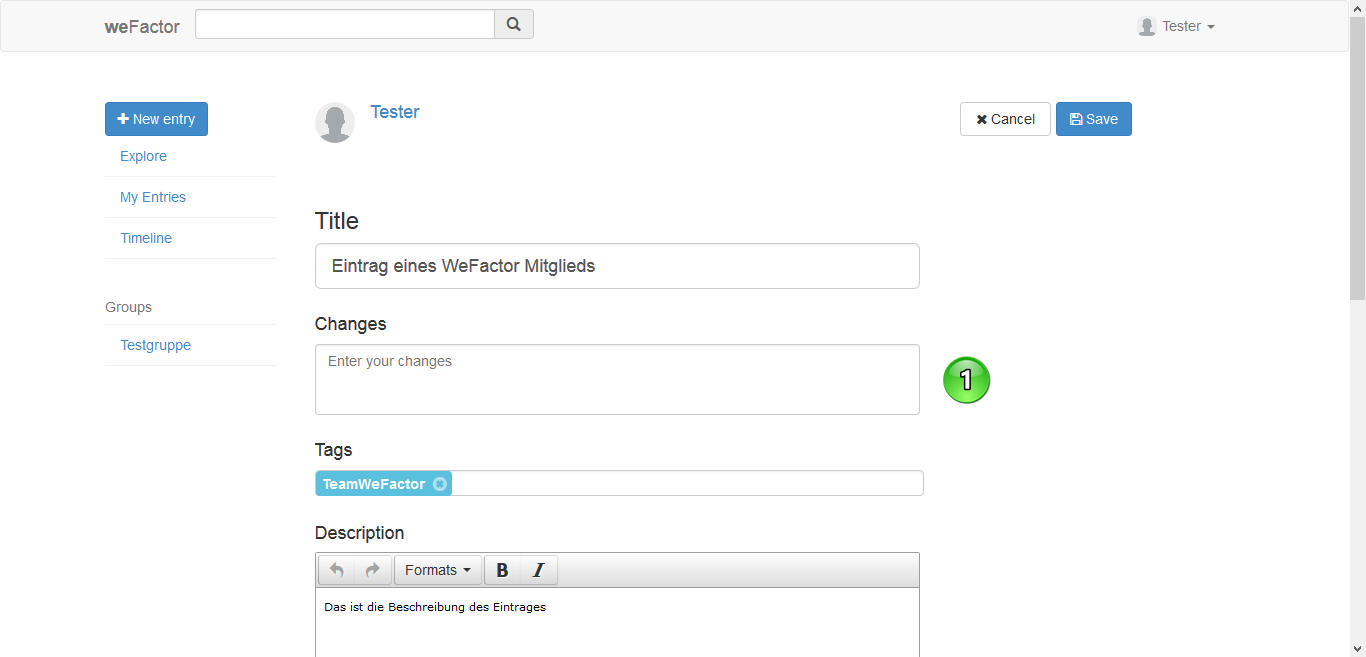
\includegraphics[width=0.8\textwidth]{Bilder/30.png}
    \caption{Versionserstellung 2}
    \label{fig:versionserstellung2}
\end{figure}
\begin{figure}[H]
    \centering
    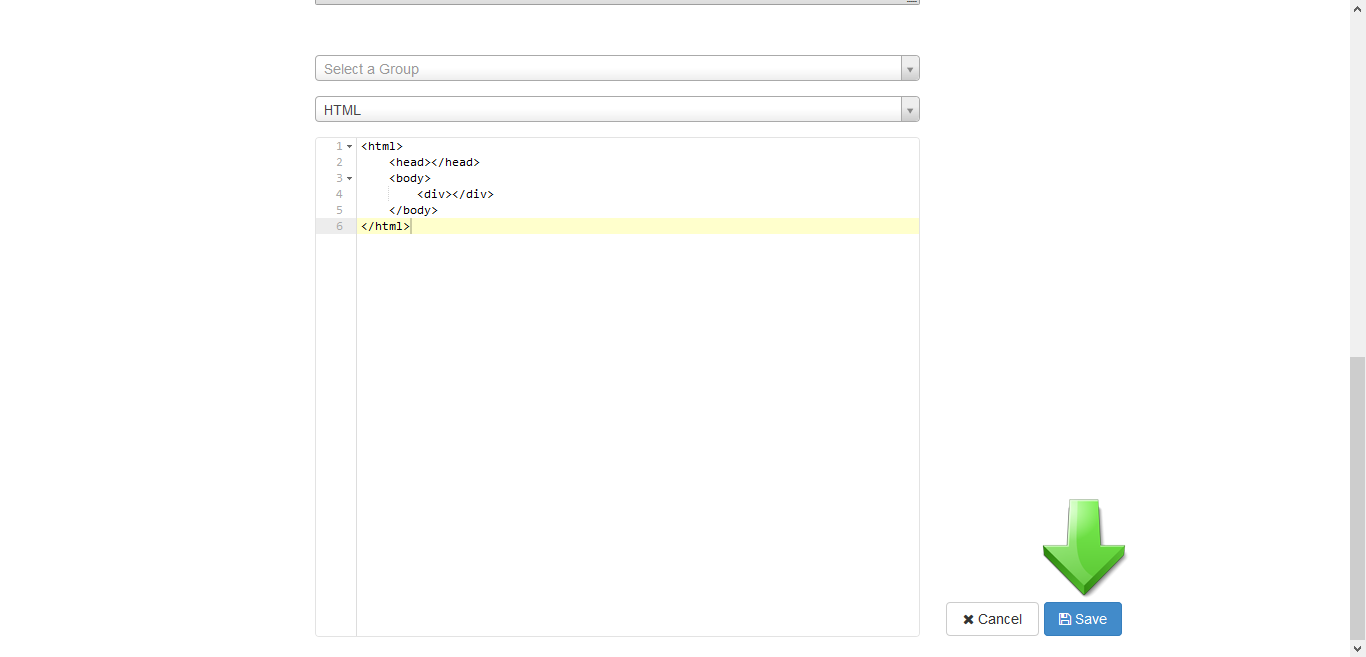
\includegraphics[width=0.8\textwidth]{Bilder/31.png}
    \caption{Versionserstellung 3}
    \label{fig:versionserstellung3}
\end{figure}


\begin{enumerate}
\item Wurde eine änderung getätigt, muss das im Textfeld „Changes“ entsprechend angegeben werden.
\end{enumerate}

Um die Erstellung des neuen Vorschlages abzuschließen, wird auf den Button „Save“ geklickt.


\section{Einen Vorschlag bekommen}

Hat der Benutzer einen Vorschlag für einen seiner Einträge bekommen, wird dies mit einer neuen Meldung in der „Timeline“ in der Navigationsbar links, wie alle anderen den Benutzer betreffenden Neuigkeiten, angezeigt.

\begin{figure}[H]
    \centering
    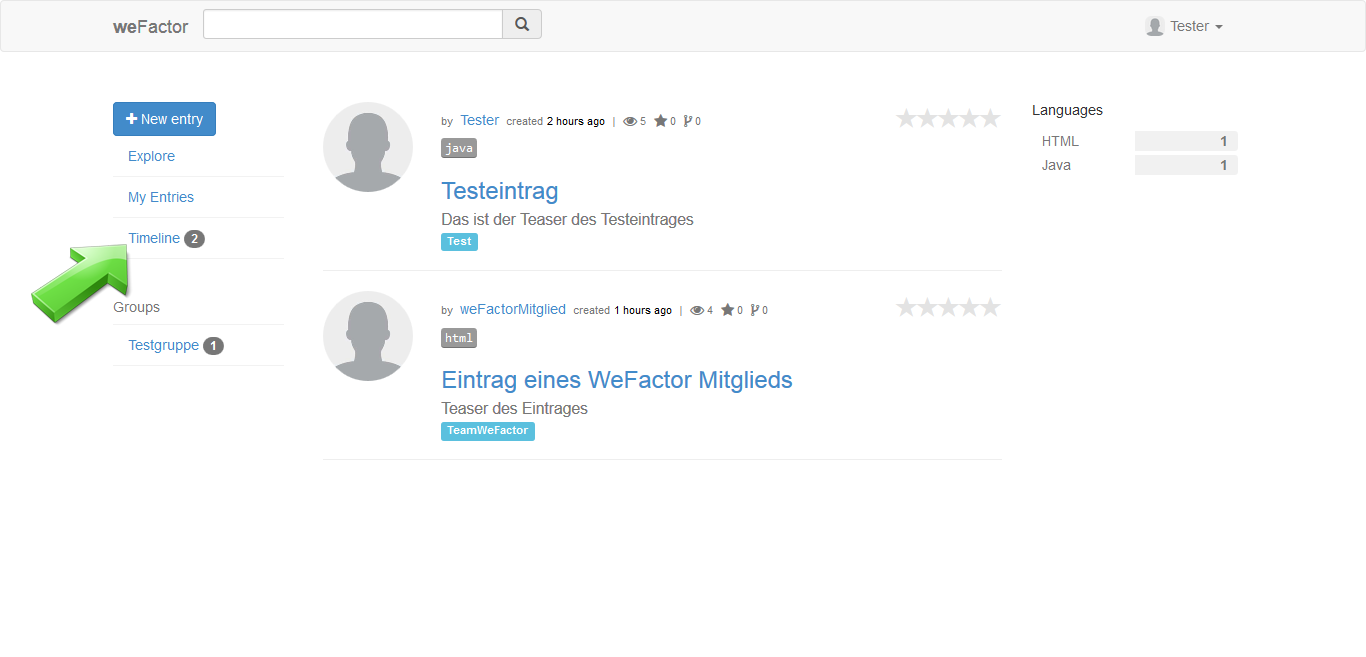
\includegraphics[width=0.8\textwidth]{Bilder/32.png}
    \caption{Exploreseite 4}
    \label{fig:exploreseite4}
\end{figure}


\subsection{Timeline, Auflistung aller des Benutzer betreffenden Neuigkeiten}

Um die Neuigkeiten anzeigen lassen zu können, klickt man in der Navigationsbar links auf „Timeline“. Zu Neuigkeiten zählen Vorschläge für Einträge des Benutzers und der Beitritt anderer Mitglieder in Gruppen, denen der Benutzer beigetreten ist.

\begin{figure}[H]
    \centering
    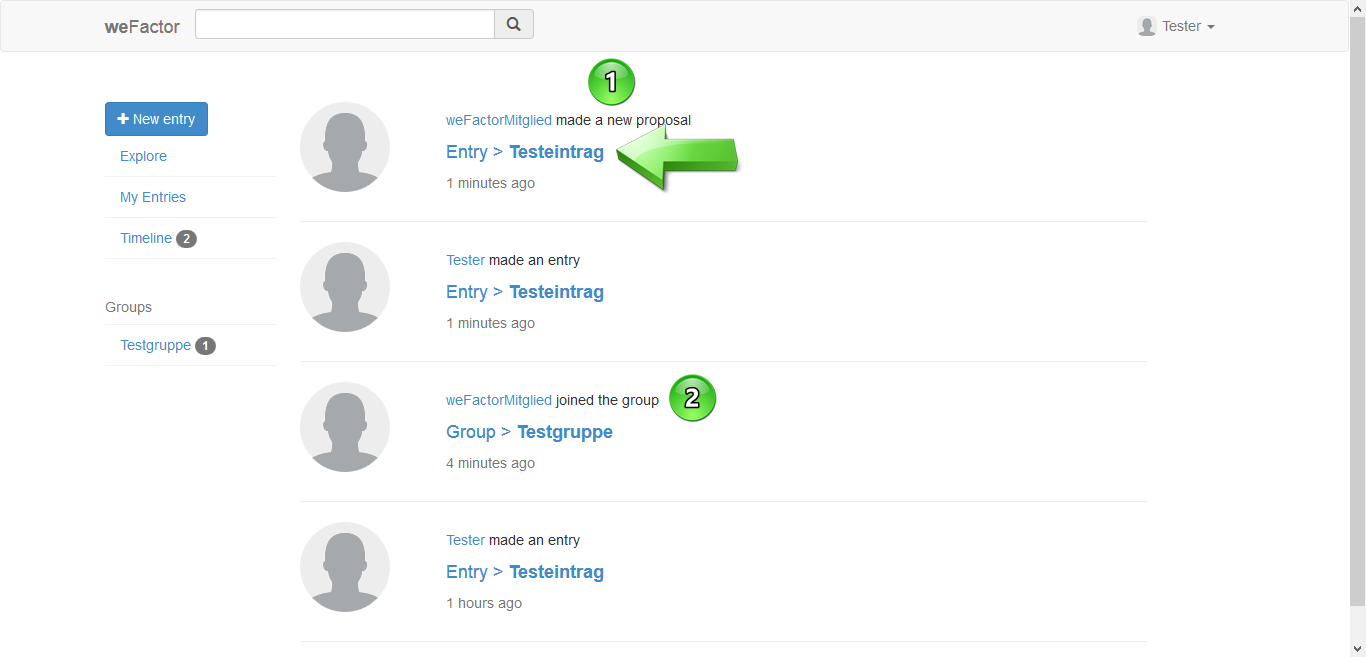
\includegraphics[width=0.8\textwidth]{Bilder/33.png}
    \caption{Timelineseite}
    \label{fig:timelineseite}
\end{figure}


Rechts vom Namen des Mitglieds wird die entsprechende Aktion angezeigt.

\begin{enumerate}
\item „made a new proposal“, es wurde ein neuer Vorschlag für den Eintrag des Benutzers erstellt.
\item „joined the group“, ein Mitglied ist der Testgruppe beigetreten.
\end{enumerate}

Als nächsten Schritt wird auf den Eintrag mit dem neuen Vorschlag geklickt.


\section{Einen Vorschlag akzeptieren/ablehnen}

Wird auf einen Eintrag mit einem neuen Vorschlag geklickt, wird man wie gewohnt auf die Eintragsübersichtsseite weitergeleitet.

\begin{figure}[H]
    \centering
    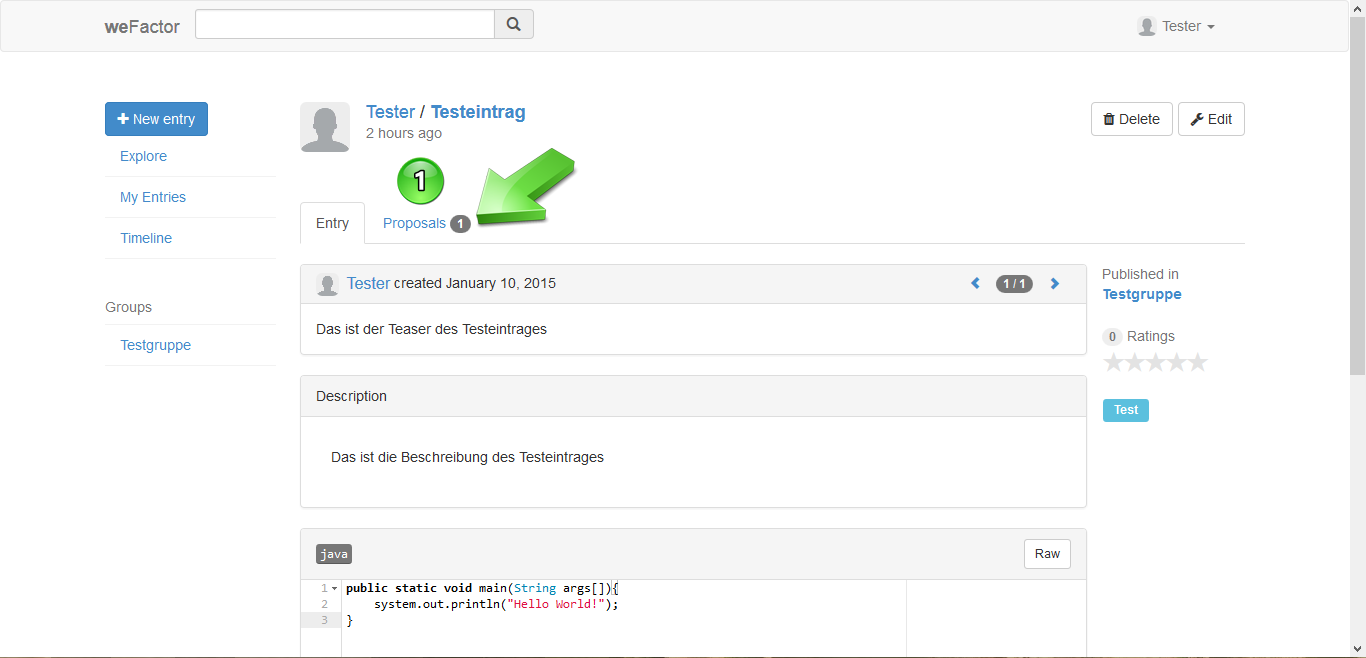
\includegraphics[width=0.8\textwidth]{Bilder/34.png}
    \caption{Eintragsuebersichtsseite 4}
    \label{fig:eintragsuebersichtsseite4}
\end{figure}


\begin{enumerate}
\item Auch hier wird mit einer entsprechenden Nummer symbolisiert, dass es einen/mehrere Vorschlag/Vorschläge für den Eintrag gibt.
\end{enumerate}


Wird auf den Reiter „Proposals“ geklickt, wird man auf die Vorschlagsübersichtsseite weitergeleitet.


\begin{figure}[H]
    \centering
    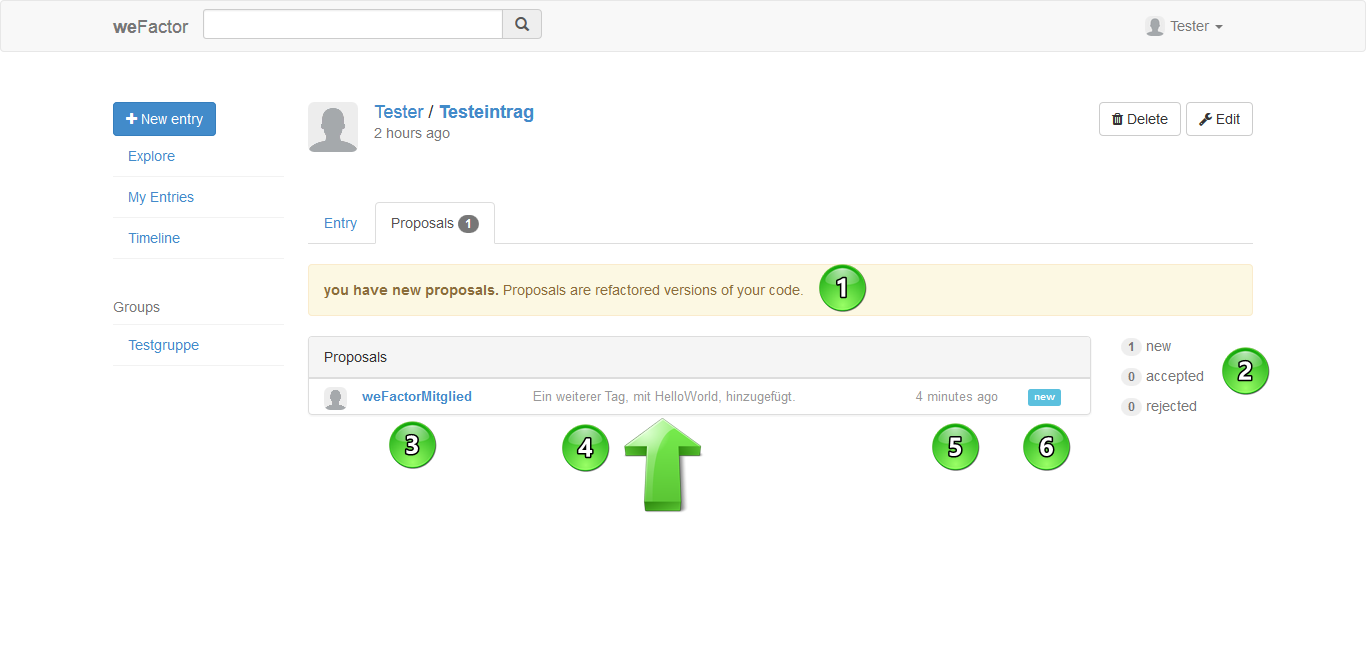
\includegraphics[width=0.8\textwidth]{Bilder/35.png}
    \caption{Vorschlaguebersichtsseite 1}
    \label{fig:vorschlaguebersichtsseite1}
\end{figure}


\begin{enumerate}
\item Informationstext, dass es neuer Vorschlag abgegeben wurde.
\item Eine übersicht, wie viele neue, akzeptierte und abgelehnte Vorschlage es gibt.
\item Name des Mitglieds, welcher den Vorschlag erstellt hat.
\item Die Beschreibung der änderung, „Changes“.
\item Zeitpunkt der Erstellung des Vorschlags.
\item Status des Vorschlags.
\end{enumerate}



Um die änderungen genauer betrachten zu können, wird auf die Beschreibung der änderung geklickt.

\begin{figure}[H]
    \centering
    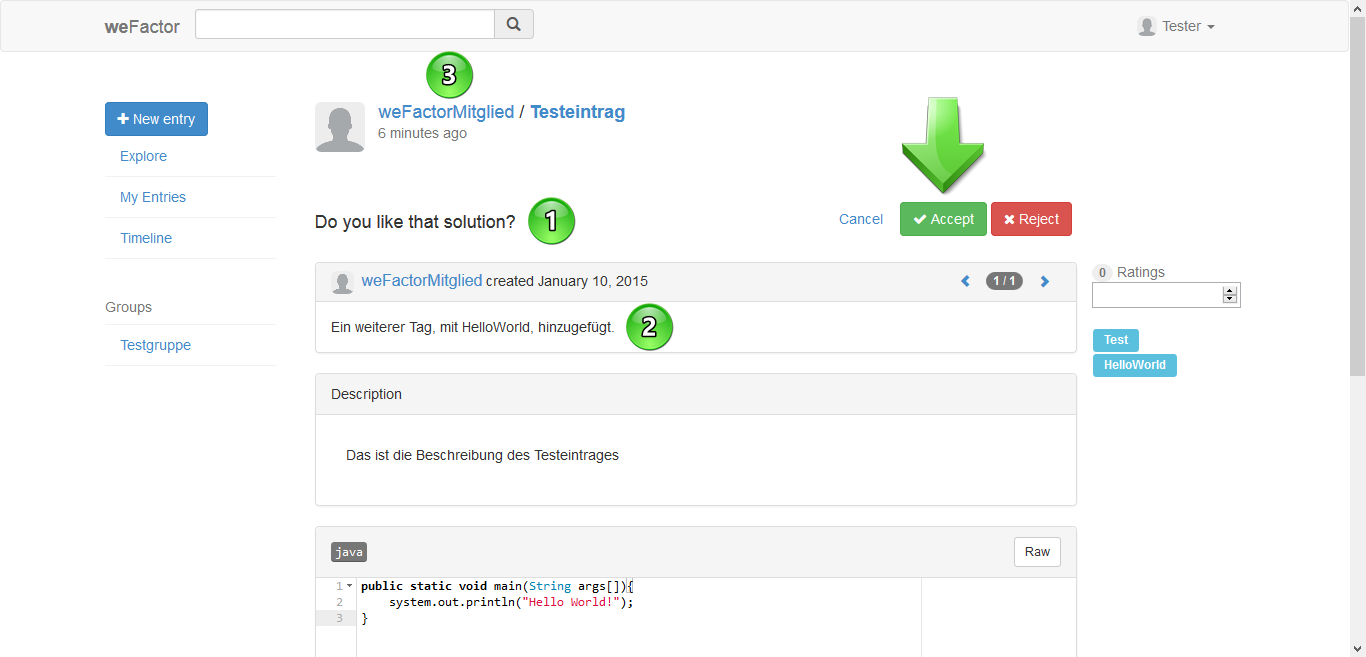
\includegraphics[width=0.8\textwidth]{Bilder/36.png}
    \caption{Vorschlaguebersichtsseite 2 }
    \label{fig:vorschlaguebersichtsseite2}
\end{figure}


\begin{enumerate}
\item Informationsmeldung ob die änderung anerkannt wird.
\item Nochmals die Angabe von Name des Mitglieds das den Vorschlag erstellt hatte, den Zeitpunkt der Erstellung und die Beschreibung der Änderung.
\item Name des Mitglieds das den Vorschlag erstellt hatte/ Name des Eintrags für den ein Vorschlag erstellt wurde.
\end{enumerate}


Nun gibt es die Möglichkeit den Vorschlag anzunehmen oder abzulehnen. Hier wird der Vorschlag akzeptiert.

\begin{figure}[H]
    \centering
    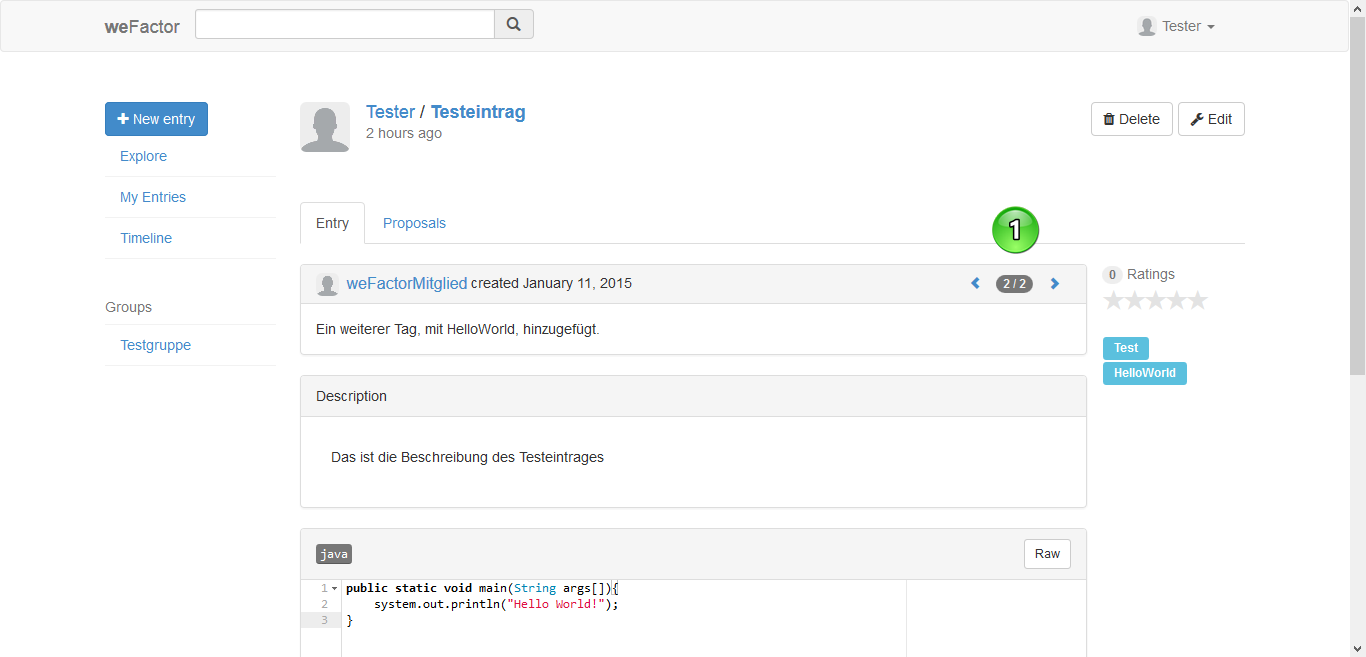
\includegraphics[width=0.8\textwidth]{Bilder/37.png}
    \caption{Vorschlagübersichtsseite 3 }
    \label{fig:vorschlaguebersichtsseite3}
\end{figure}


Wird der Vorschlag akzeptiert wird man auf die Eintragsübersichtsseite weitergeleitet. Hier gibt es nun die Möglichkeit zwischen den verschieden Versionen zu wechseln.

\begin{enumerate}
\item Anzahl der Versionen die es für diesen Eintrag gibt. Zwischen den Versionen kann beliebig gewechselt werden.
\end{enumerate}


Als nächsten Schritt wird für einen beliebigen Eintrag eine Bewertung abgegeben.



\chapter{Eine Bewertung abgegeben}

Bewertungen können von eins bis fünf Sterne abgegeben werden.
Auf der „Explore“-Seite wird ein beliebiger Eintrag gewählt und auf ihn geklickt.

\begin{figure}[H]
    \centering
    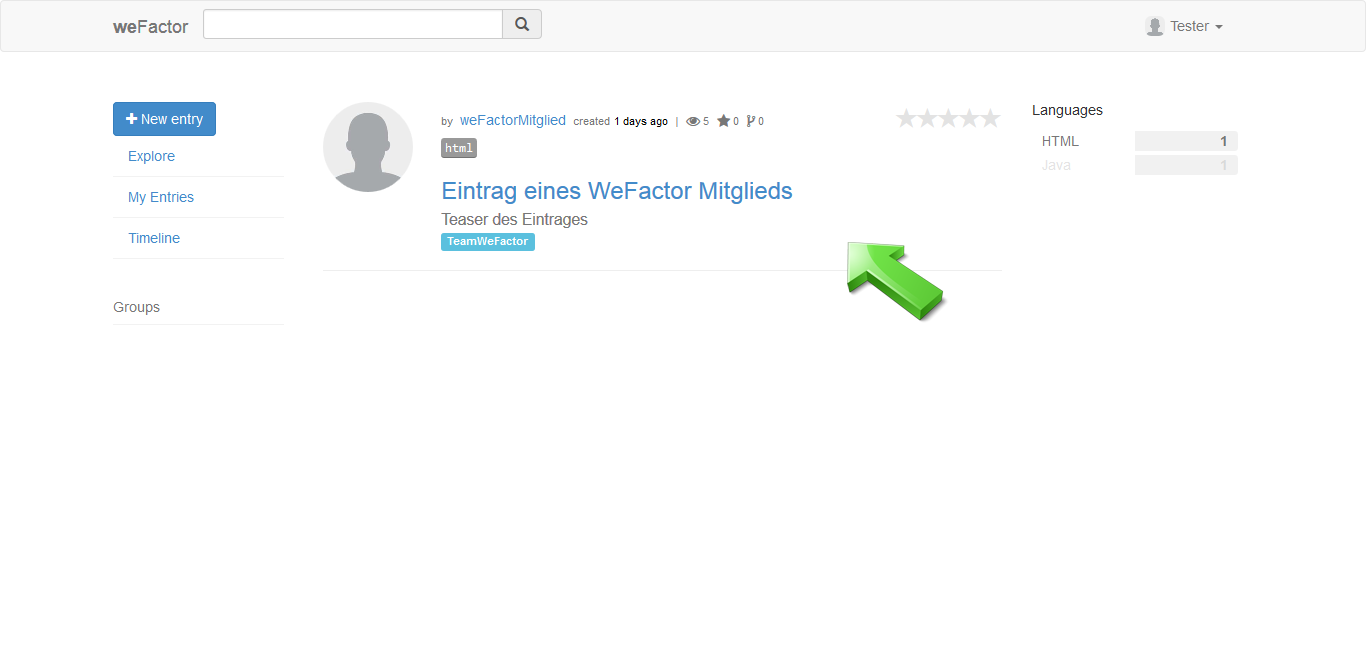
\includegraphics[width=0.8\textwidth]{Bilder/40.png}
    \caption{Exploreseite 5 }
    \label{fig:exploreseite5}
\end{figure}


Wird auf einen Eintrag geklickt, wird man auf die Eintragsübersichtsseite weitergeleitet.

\begin{figure}[H]
    \centering
    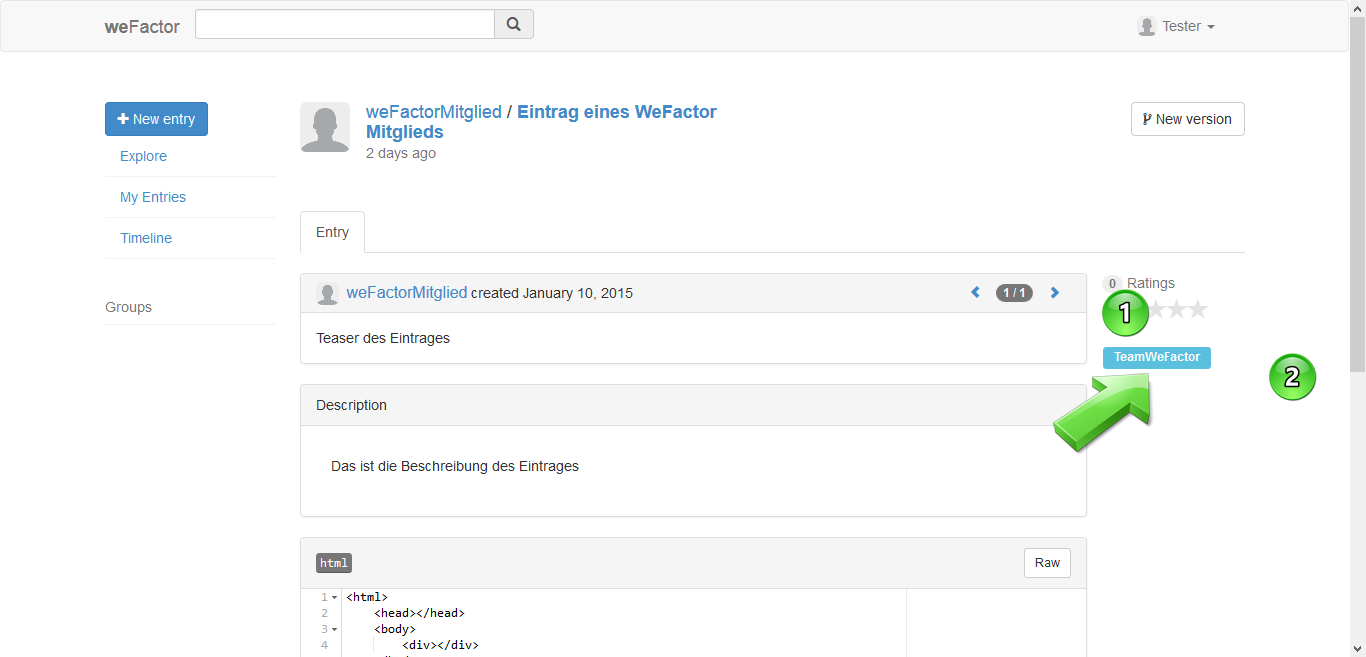
\includegraphics[width=0.8\textwidth]{Bilder/41.png}
    \caption{Bewertung 1}
    \label{fig:bewertung1}
\end{figure}


\begin{enumerate}
\item Anzahl der bisherigen Bewertungen.
\item Mit Klicken auf die gewünschte Anzahl der Sterne kann die Bewertung abgegeben werden.
\end{enumerate}


\begin{figure}[H]
    \centering
    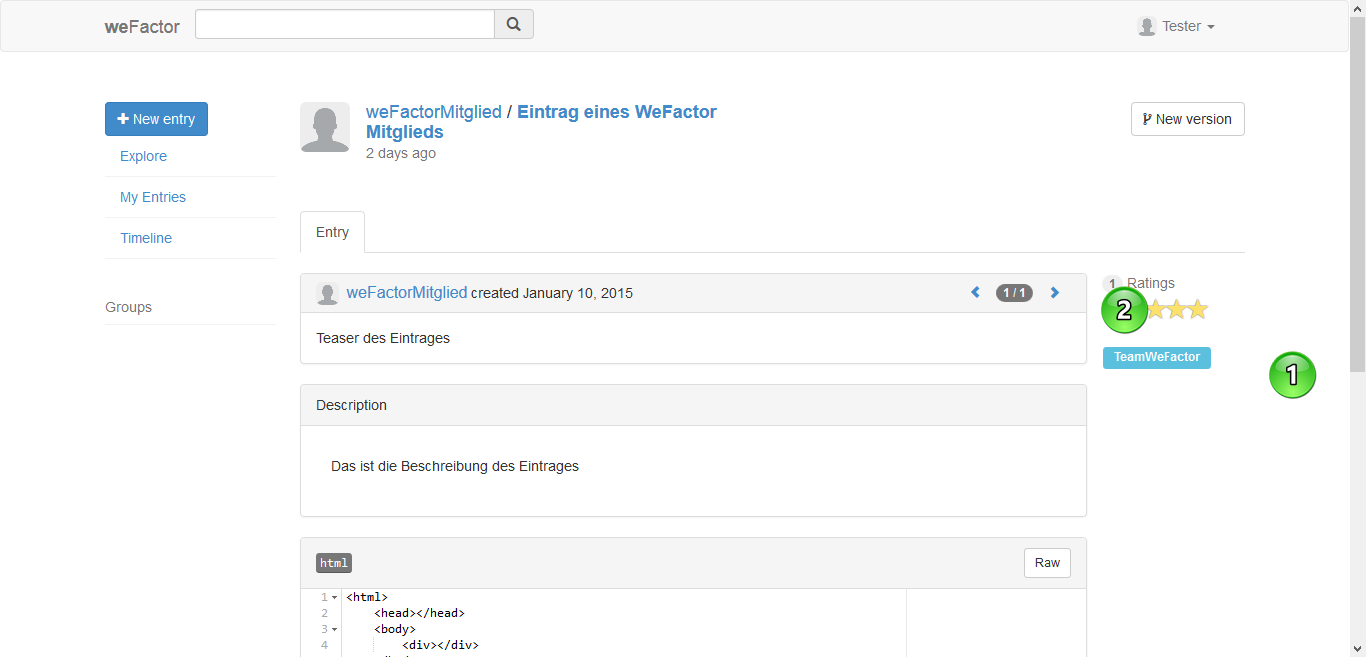
\includegraphics[width=0.8\textwidth]{Bilder/42.png}
    \caption{Bewertung 2}
    \label{fig:bewertung2}
\end{figure}


\begin{enumerate}
\item Es wurde eine 5-Sterne Bewertung abgegeben.
\item Es wurde nun insgesamt eine Bewertung abgegeben.
\end{enumerate}














% Literaturverzeichnis
%
% Dokumentation
%

% Kapitel dem Inhaltsverzeichnis hinzufügen
%\addcontentsline{toc}{chapter}{Literaturverzeichnis}			% 1. Argument {toc} = Table Of Contents
																% 2. Argument {chapter} = Ebene bestimmen!
																% 3. Argument {Name} = Name des Eintrags
\noindent

\thispagestyle{plain}

%\chapter*{Literaturverzeichnis}
\bibliographystyle{apacite}
\bibliography{techDoku}  % Bibtex-Datei wird schon in der Preambel eingebunden





% Anhang
%\include{16_Anhang}

\end{document}